\documentclass[Bachelorarbeit.tex]{subfiles}
\begin{document}

\graphicspath{{./figures/newMarket/}}	%specifying the folder for the figures

\chapter{A new Market}
As already introduced in chapter \ref{ch:interpretation} "Interpretation" a new market is necessary to repair the miss-allocation of collateralized assets in the range of the pessimist agents by enabling the agents to trade collateralized assets against cash.

\section{Implementation}

\subsection{Price-Range}
As for all other 3 Markets the price-ranges of the offers must be defined. Note that all prices must obviously be in the unit of cash.

\paragraph{minimum}
When calculating the minimum price of a collateralized asset - that is how much is the collateralized asset minimally worth - it is important to include the collateral-aspect of the asset. Thus one starts with the minimum asset-price in cash which is the down-price \textit{pD} and subtracts the maximum possible amount of cash which is bound through a bond as collateral which is the face-value \textit{V}. This value is a constant for all agents.

\begin{center}
$\textit{min collateralized asset-price} = \min(0, \textit{pD} - \textit{V})$
\end{center}
 
\paragraph{maximum}
To calculate the maximum price of a collateralized asset - that is how much is the collateralized asset maximally worth - one needs to include the collateral-aspect of the asset too. Equal to calculating the minimum one starts now with the maximum asset-price in cash which is the up-price \textit{pU} and subtracts the minimum possible amount of cash which is bound through a bond as collateral which is the face-value \textit{pD}. This value is a constant for all agents.

\begin{center}
$\textit{max collateralized asset-price} = \textit{pU} - \textit{pD}$
\end{center}

\paragraph{limit}
Applying the same rules as in minimum and maximum to the limit price calculation one needs to subract the limit-price of loans from the limit-price of asset to receive the limit-price of a collateralized asset. This value is individual for each agent as the limit-prices differ across the agents both for assets and loans.

\begin{center}
$\textit{limit-price of collateralized asset} = \textit{limit-price of asset} - \textit{limit-price of loan}$
\end{center}

\subsection{Bid-Offering}
The way bid-offers are generated is very similar to the "Bond against Cash" market. Bid Offerings are generated only when the agent has any cash holdings. The price is drawn randomly between the minimum price and the limit-price because when buying one wants to buy below the expected value to make a profit. As amount one TRADING-UNIT of an asset is selected - in the thesis-implementation 0.1 - but if there is not enough cash left to buy one TRADING-UNIT of assets then the amount of assets is selected which can be bought with the remaining cash holdings.

\begin{table}[H]
	\centering
	\caption{Bid-Offering parameters}
	\begin{tabular} { l c r }
		\hline
		Pre-Condition & $\textit{cash holdings} > 0$  \\
		Asset-Price & $\mathrm{random}(\textit{min coll. asset-price}, \textit{limit-price of coll. asset})$ \\
		Asset-Amount & $\min ( \frac{ \textit{cash holdings} }{ \textit{Asset-Price} }, \textit{TRADING-UNIT} )$ \\
		\hline
	\end{tabular}
\end{table}


\subsection{Ask-Offering}
The way ask-offers are generated is very similar to the "Bond against Cash" market. Ask Offerings are generated only when the agent has any collateralized assets. The price is drawn randomly between the limit-price and maximum price because when selling one wants to sell above the expected value to make a profit. As amount one TRADING-UNIT of an asset is selected - in the thesis-implementation 0.1 - but if there are fewer collateralized assets left then the remaining amount of collateral is selected.

See Chapter \ref{ch:implementation} "Implementation" for the equation of collateral holdings.

\begin{table}[H]
	\centering
	\caption{Ask-Offering parameters}
	\begin{tabular} { l c r }
		\hline
		Pre-Condition & $\textit{collateral holdings} > 0$  \\
		Asset-Price & $\mathrm{random}(\textit{limit-price of coll. asset}, \textit{max coll. asset-price})$ \\
		Asset-Amount & $\min ( { \textit{collateral holdings} }, \textit{TRADING-UNIT} )$ \\
		\hline
	\end{tabular}
\end{table}

\subsection{Match}
Below the wealth-exchange table is given in case of a match between two agents on the new market.

\begin{table}[H]
	\centering
	\caption{Wealth-Exchange on match}
	\begin{tabular} { l c c }
		& Seller & Buyer \\
		\hline
		Loan Given & + matching-amount & N/A \\
		Loans Taken & N/A & - matching-amount \\
		Assets holdings & - matching-amount & + matching-amount \\
		Cash holdings  & + matching-price & - matching-price \\
		\hline
	\end{tabular}
\end{table}

\section{Results}
Of most importance are the results of the simulation when using the new market. The plain results are given in this section where the interpretation of the results are given in the following section.

\medskip

As experiment-configuration the same is used as given in Chapter \ref{ch:results} "Results" except that the new market is now activated too.

\subsection{Fully-Connected topology}
\begin{table}[H]
	\centering
	\caption{Configuration for all experiments}
	\begin{tabular} { l c r }
		\hline
		Agent-Count & 100 \\
		Bond-Type & 0.5 \\
		Replication-Count & 50 \\
		Terminate after & 1000 failed successive Transactions \\
		\hline
	\end{tabular}
\end{table}

\begin{figure}[H]
	\centering
  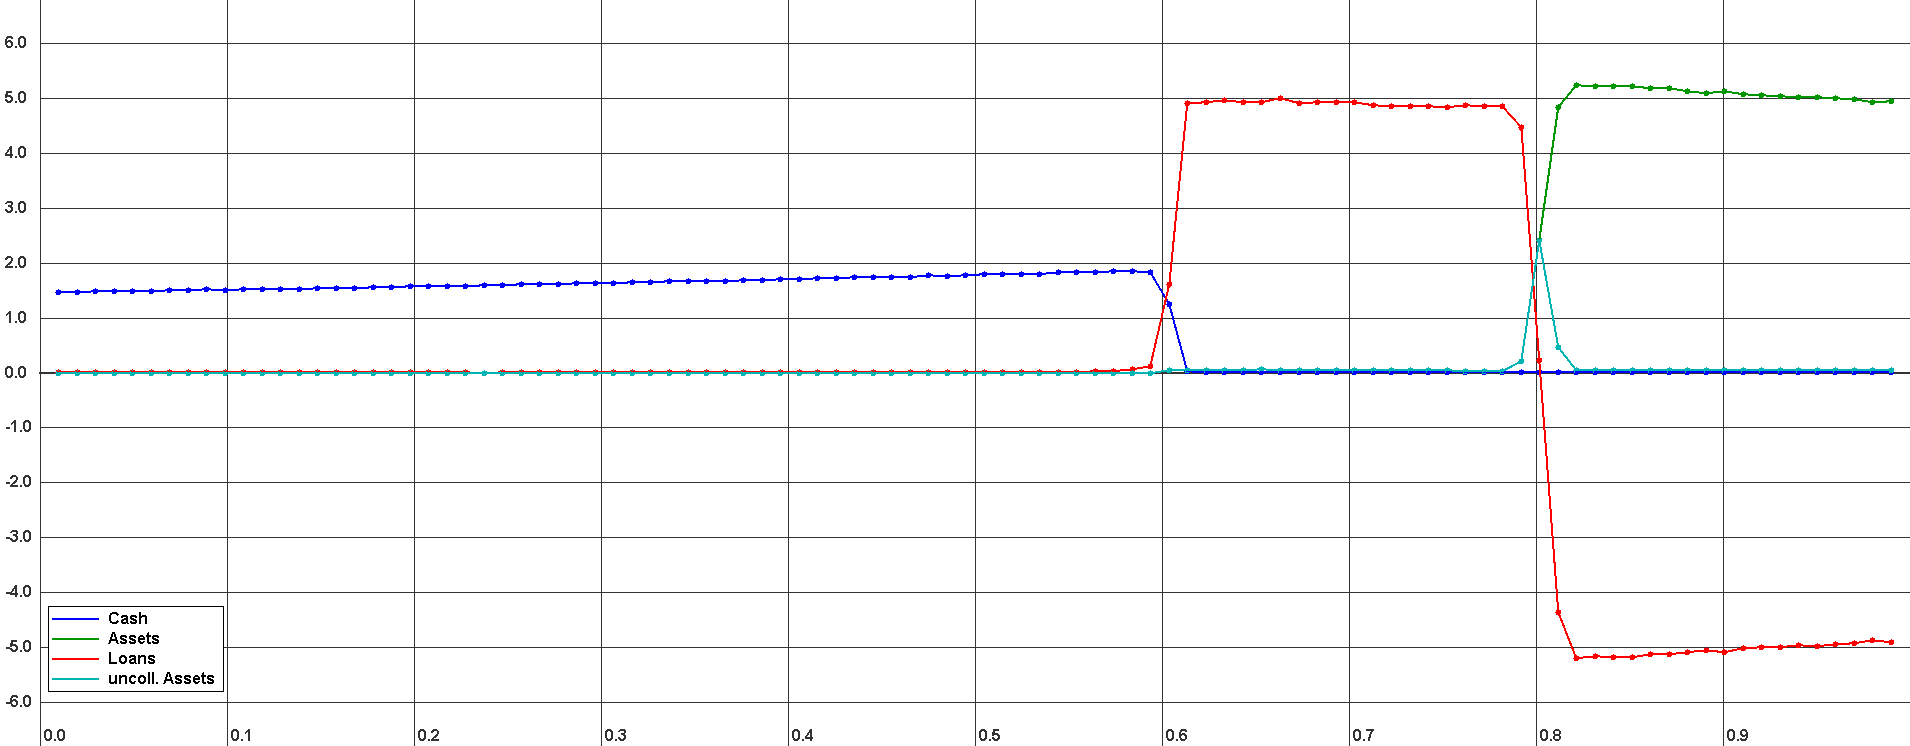
\includegraphics[width=1.0\textwidth, angle=0]{FULLYCONNECTED_100_WITHCOLLATERALMARKET_REPL.png}
	\caption{Wealth-Distribution of Fully-Connected topology with collateral/cash market}
	\label{fig:wealth_FULLYCONNECTED_100_WITHCOLLATERALMARKET_REPL}
\end{figure}

\begin{table}[H]
	\caption{Equilibrium of Fully-Connected topology with collateral/cash market}
	\centering
	\begin{tabular} { l c r }
		\hline
		Asset-Price & 0.688 (0.008) \\
		Loan-Price & 0.381 (0.002) \\
		Marginal Buyer i0 & 0.597 (0.005) \\
		Marginal Seller i1 & 0.803 (0.003) \\
		\hline
		Pessimist Wealth & 1.597 (0.009) \\
		Medianist Wealth & 4.76 (0.1) \\
		Optimist Wealth & 4.963 (0.052) \\
		\hline
	\end{tabular}
\end{table} 

\begin{table}[H]
	\caption{Performance of Fully-Connected topology with collateral/cash market}
	\centering
	\begin{tabular} { l c r }
		\hline
		Successful TX & 1916.14 (31.42) \\
		Total TX & 6364.8 (1679.21) \\
		Failed TX & 4448.66 (1668.93) \\
		\hline
	\end{tabular}
\end{table}

TODO: irgendeine statistischer test, der anhand mittelwert und standardabweichung vergleichen lässt?
T-Test und F-Test.
aber kommen kaum vernünftige werte heraus

\begin{table}[H]
	\caption{Difference of Fully-Connected topology to theoretical equilibrium as given in Table \ref{tab:theoretical_equilibrium_100Agents_05Bond} of Chapter \ref{ch:results} "Results"}
	\centering
	\begin{tabular} { l c c c r }
		& Result & Reference & difference to Reference \\
		\hline
		Asset-Price & 0.688 & 0.717 & -4.0\% \\
		Loan-Price & 0.381 & 0.375 & +1.6\% \\
		Marginal Buyer i0 & 0.597 & 0.584 & +2.2\% \\
		Marginal Seller i1 & 0.802 & 0.803 & +0.1\% \\
		\hline
	\end{tabular}
\end{table} 

\begin{table}[H]
	\caption{Difference of Fully-Connected topology to equilibrium without collateral/cash market as given in Table \ref{tab:fullyconnected_equilibrium_100Agents_05Bond} of Chapter \ref{ch:results} "Results"}
	\centering
	\begin{tabular} { l c c c r }
		& Result & Reference & difference to Reference \\
		\hline
		Asset-Price & 0.688 & 0.689 & -0.1\% \\
		Loan-Price & 0.381 & 0.384 & -0.7\% \\
		Marginal Buyer i0 & 0.597 & -0.006 & -1.0\% \\
		Marginal Seller i1 & 0.803 & 0.803 & 0.0\% \\
		\hline
		Pessimist Wealth & 1.597 & 1.597 & 0.0\% \\
		Medianist Wealth & 4.76 & 4.565 & +4.2\% \\
		Optimist Wealth & 4.963 & 5.02 & -1.1\% \\
		\hline
	\end{tabular}
\end{table} 

TODO: irgendeine statistischer test, der anhand mittelwert und standardabweichung vergleichen lässt?
T-Test und F-Test.
aber kommen kaum vernünftige werte heraus


\subsection{Ascending-Connected topology}
\begin{figure}[H]
	\centering
  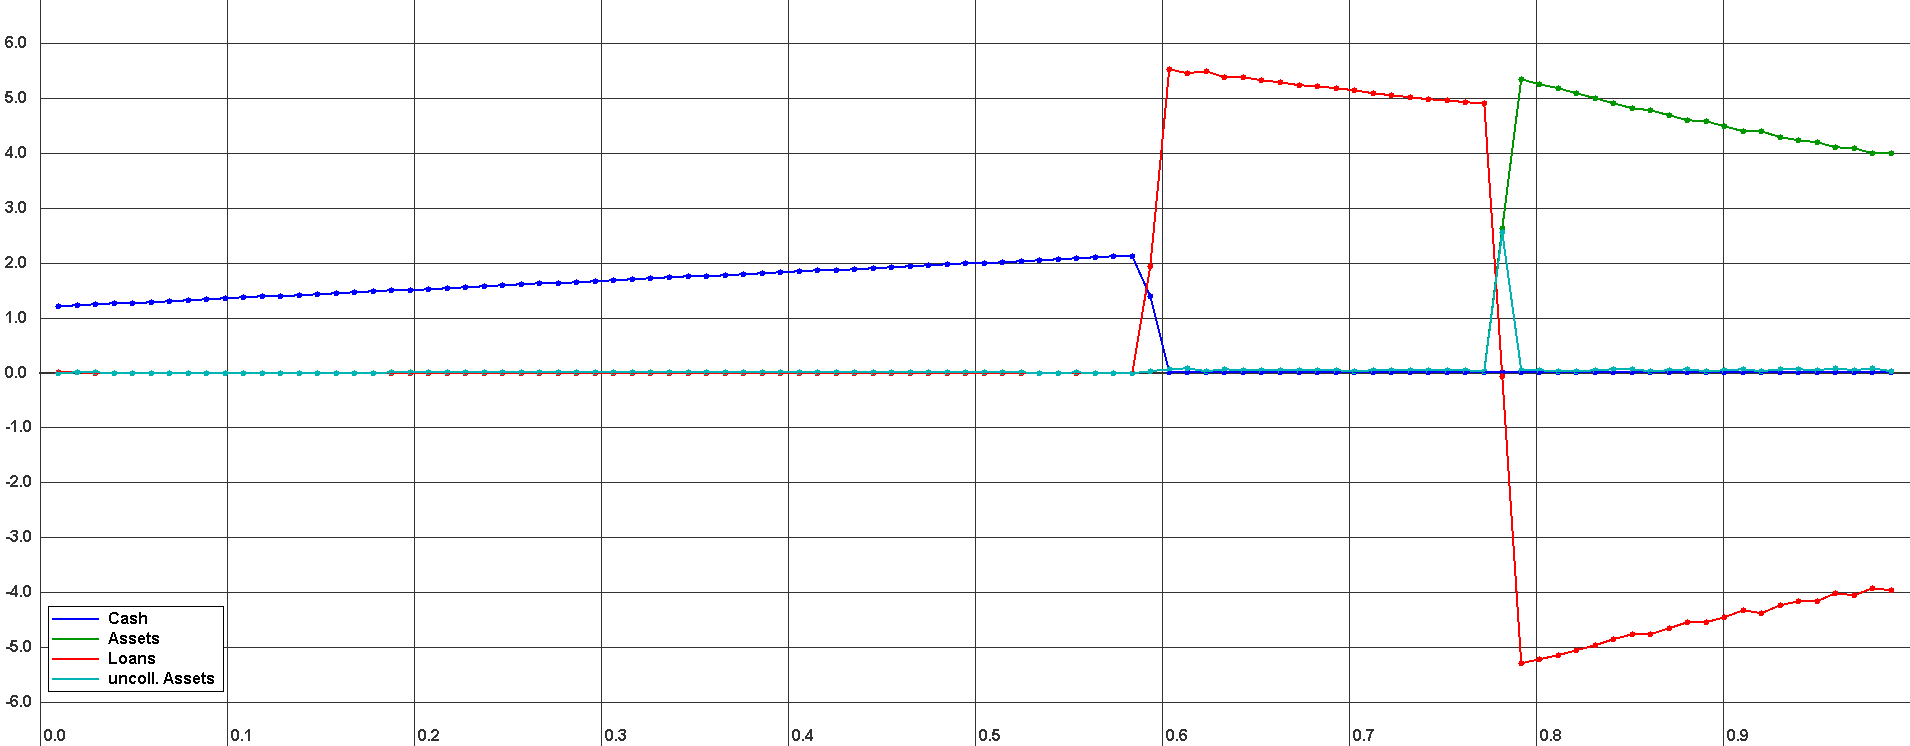
\includegraphics[width=1.0\textwidth, angle=0]{ASCENDINGCONNECTED_100_WITHCOLLATERALMARKET_REPL.png}
	\caption{Wealth-Distribution of Ascending-Connected topology with collateral/cash market}
	\label{fig:wealth_ASCENDINGCONNECTED_100_WITHCOLLATERALMARKET_REPL}
\end{figure}

\begin{table}[H]
	\caption{Equilibrium of Ascending-Connected topology}
	\centering
	\begin{tabular} { l c r }
		\hline
		Asset-Price & 0.713 (0.013) \\
		Loan-Price & 0.383 (0.005) \\
		Marginal Buyer i0 & 0.584(0.0) \\
		Marginal Seller i1 & 0.782 (0.0) \\
		\hline
		Pessimist Wealth & 1.671 (0.0) \\
		Medianist Wealth & 5.032 (0.013) \\
		Optimist Wealth & 4.508 (0.006) \\
		\hline
	\end{tabular}
\end{table} 

\begin{table}[H]
	\caption{Performance of Ascending-Connected topology}
	\centering
	\begin{tabular} { l c r }
		\hline
		Successful TX & 51,838.74 (1613.36) \\
		Total TX & 52.963.5 (1612.31) \\
		Failed TX & 1124.76 (28.31) \\
		\hline
	\end{tabular}
\end{table}

\begin{table}[H]
	\caption{Difference of Ascending-Connected topology to theoretical equilibrium as given in Table \ref{tab:theoretical_equilibrium_100Agents_05Bond} of Chapter \ref{ch:results} "Results"}
	\centering
	\begin{tabular} { l c c c r }
		& Result & Reference & difference to Reference \\
		\hline
		Asset-Price & 0.713 & 0.717 & -0.5\% \\
		Loan-Price & 0.383 & 0.375 & +2.1\% \\
		Marginal Buyer i0 & 0.584 & 0.584 & 0.0\% \\
		Marginal Seller i1 & 0.782 & 0.802 & -2.5\% \\
		\hline
	\end{tabular}
\end{table} 

TODO: irgendeine statistischer test, der anhand mittelwert und standardabweichung vergleichen lässt?
T-Test und F-Test.
aber kommen kaum vernünftige werte heraus


\begin{table}[H]
	\caption{Difference of Ascending-Connected topology to equilibrium without collateral/cash market as given in Table \ref{tab:ascendingconnected_equilibrium_100Agents_05Bond} of Chapter \ref{ch:results} "Results"}
	\centering
	\begin{tabular} { l c c c r }
		& Result & Reference & difference to Reference \\
		\hline
		Asset-Price & 0.713 & 0.711 & +0.3\% \\
		Loan-Price & 0.383 & 0.391 & -2.0\% \\
		Marginal Buyer i0 & 0.584 & 0.646 & -9.6\% \\
		Marginal Seller i1 & 0.782 & 0.85 & -8.0\% \\
		\hline
		Pessimist Wealth & 1.671 & 1.166 & +43.3\% \\
		Medianist Wealth & 5.032 & 1.869 & +169.2\% \\
		Optimist Wealth & 4.508 & 4.307 & +4.6\% \\
		\hline
	\end{tabular}
\end{table}

TODO: irgendeine statistischer test, der anhand mittelwert und standardabweichung vergleichen lässt?
T-Test und F-Test.
aber kommen kaum vernünftige werte heraus

\begin{table}[H]
	\caption{Difference of Ascending-Connected to equilibrium of fully-connected topology with collateral/cash market as given above}
	\centering
	\begin{tabular} { l c c c r }
		& Result & Reference & difference to Reference \\
		\hline
		Asset-Price & 0.713 & 0.688 & +3.6\% \\
		Loan-Price & 0.383 & 0.381 & +0.5\% \\
		Marginal Buyer i0 & 0.584 & 0.597 & -2.2\% \\
		Marginal Seller i1 & 0.782 & 0.803 & -2.6\% \\
		\hline
		Pessimist Wealth & 1.671 & 1.597 & +4.6\% \\
		Medianist Wealth & 5.032 & 4.76 & +5.7\% \\
		Optimist Wealth & 4.508 & 4.963 & -9.2\% \\
		\hline
	\end{tabular}
\end{table}

TODO: irgendeine statistischer test, der anhand mittelwert und standardabweichung vergleichen lässt?
T-Test und F-Test.
aber kommen kaum vernünftige werte heraus


\begin{table}[H]
	\caption{Difference of Ascending-Connected to equilibrium of fully-connected without collateral/cash market as given in Table \ref{tab:fullyconnected_equilibrium_100Agents_05Bond} of Chapter \ref{ch:results} "Results"}
	\centering
	\begin{tabular} { l c c c r }
		& Result & Reference & difference to Reference \\
		\hline
		Asset-Price & 0.713 & 0.689 & +3.5\% \\
		Loan-Price & 0.383 & 0.384 & -0.3\% \\
		Marginal Buyer i0 & 0.584 & 0.603 & -3.2\% \\
		Marginal Seller i1 & 0.782 & 0.803 & -2.6\% \\
		\hline
		Pessimist Wealth & 1.671 & 1.597 & +4.6\% \\
		Medianist Wealth & 5.032 & 4.565 & +10.23\% \\
		Optimist Wealth & 4.508 & 5.021 & -10.22\% \\
		\hline
	\end{tabular}
\end{table} 

TODO: irgendeine statistischer test, der anhand mittelwert und standardabweichung vergleichen lässt?
T-Test und F-Test.
aber kommen kaum vernünftige werte heraus


\section{Interpretation of results}
Interpreting the results the following questions must be answered:

\begin{itemize}
\item Does the Fully-Connected topology reach the theoretical equilibrium as well?
\item Does the new market repair the miss-allocation of wealth in the pessimists-range?
\item If not why? If yes, does the Ascending-Connected topology approach theoretical equilibrium now?
\end{itemize}

\paragraph{Does the Fully-Connected topology reach the theoretical equilibrium as well?}
Yes it does. Both visual and statistical results show that it reaches the theoretical equilibrium. The medianist wealth is slightly higher with the new market but that difference, as well as the variations in the other variables are not statistically significant. TODO: genauer.

\paragraph{Does the new market repair the miss-allocation of wealth in the pessimists-range?}
Yes it does. The visual results are clear: no more miss-allocations show up within 50 replications.

\paragraph{If yes, does the Ascending-Connected topology approach theoretical equilibrium now?}
No it does not. Both visual and statistical results show that it misses to reach the theoretical and fully-connected topology with/without new market equilibrium: genauer.
Clearly the visual and statistical results are different than in the case without the new market but that was expected and is a necessity if the new market repairs the miss-allocation of wealth in the pessimists-range. TODO: genauer.


\section{Simulation and Market dynamics}
When implementing a new market the market-dynamics are of very importance and thus the following questions must be answered.

\begin{itemize}
\item Can the trading stages 1-4 be identified too as given in \cite{Breuer_2015}?
\item How does trading progress with this new market? Is it the same as without the new market?
\item How does the new market resolve the miss-allocation (turning on after no more possible)?
\item When and how much is each market active? 
\item How do the market-activities change when a new market is introduced?
\end{itemize}

To answer these questions one must look closely at the market-dynamics. There are definitely trading stages but due to the new market or the different topology they are expected to be quite different from the ones found in \cite{Breuer_2015}. The method used to find these stages is through observation of a single run and refining and validating the derived facts over many additional runs. Note that replications provide no real value here as one needs to look very carefully into the dynamics of single runs instead of the mean of multiple runs.

\subsection{Fully-Connected with new Market}

4 Stages were identified which are quite different from the ones given in \cite{Breuer_2015}.

\begin{figure}[H]
	\centering
  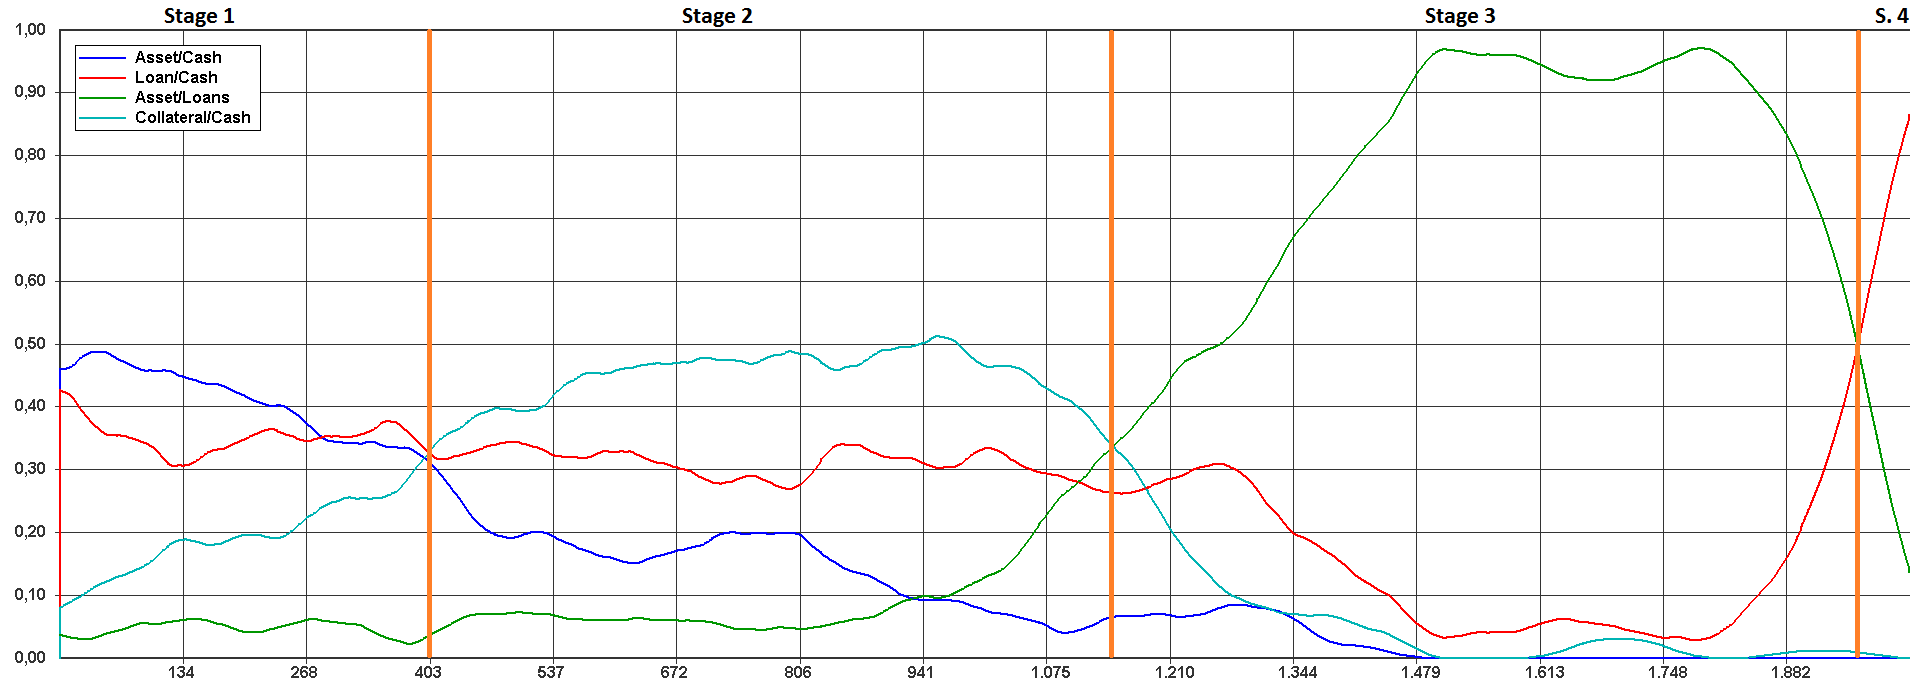
\includegraphics[width=1.0\textwidth, angle=0]{fc/FULLYCONNECTED_100_WITHCOLLATERALMARKET_MARKET_STAGES.png}
  	\caption{Market-activity stages of Fully-Connected topology with collateral/cash market}
	\label{fig:markets_FULLYCONNECTED_100_WITHCOLLATERALMARKET_MARKET_STAGES}
\end{figure}

\paragraph{Stage 1}
In this stage the pessimists become visible rapidly as they sell their assets and increase their cash wealth. One can get also a sense of the more optimistic range of agents as they gather assets both free and collateralized. The medianists are not visible yet.

\medskip

The asset/cash market dominates but goes down slowly as fewer and fewer pessimists trade assets against cash compared to the very beginning. 
The loan/cash market fluctuates around the same point as loans are traded more or less equally the same.
The collateral/cash market begins quite low and raises as more and more collateralized assets are created by pessimists and need to be sold again using the new market.
The asset/loan market is hardly active as there is no strong need for its features yet.

\begin{figure}[H]
	\centering
  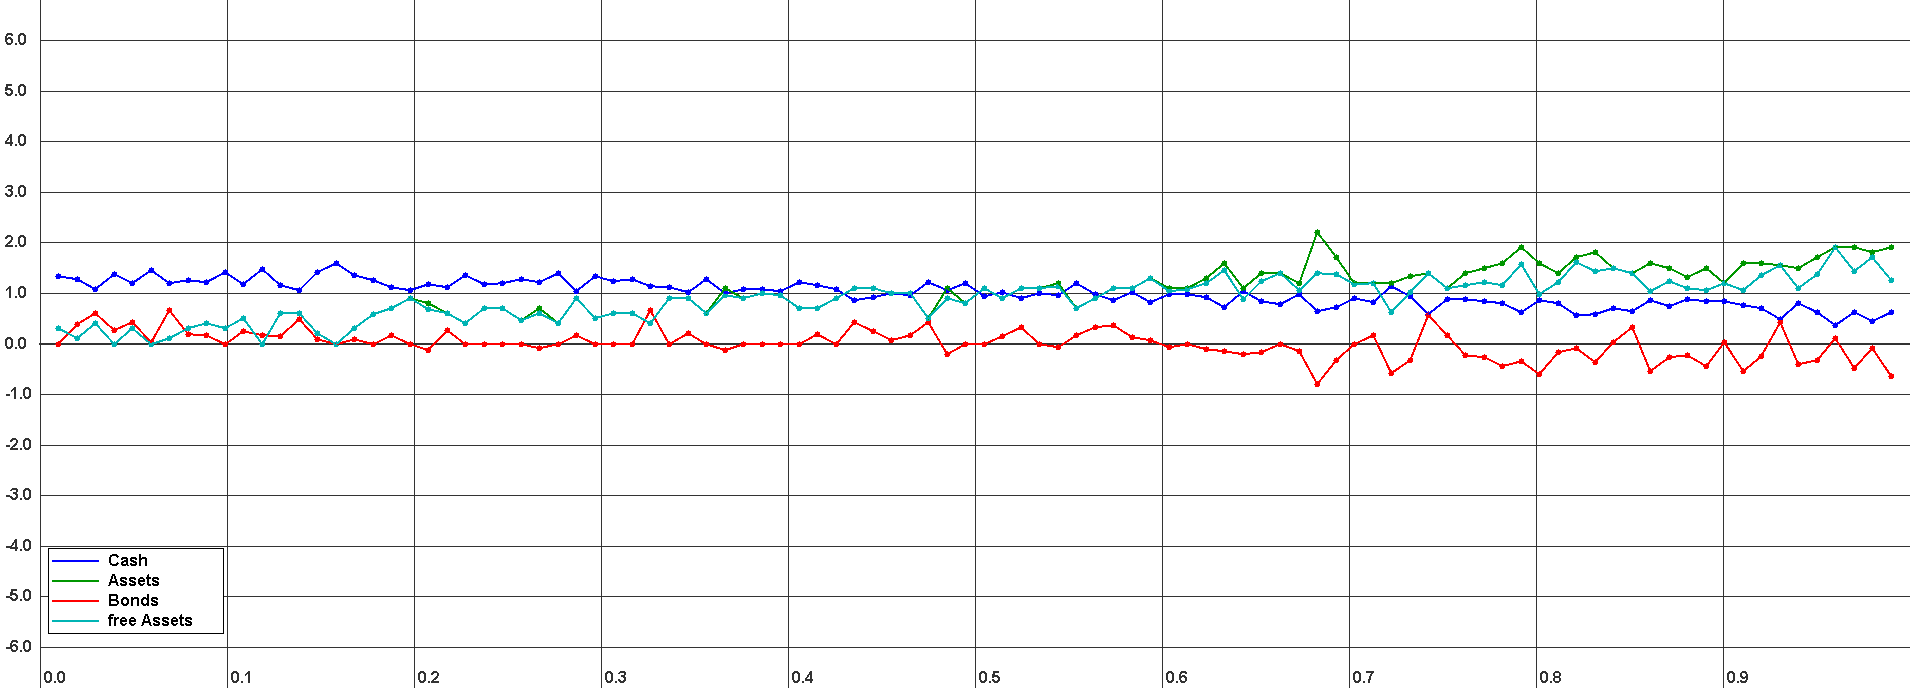
\includegraphics[width=1.0\textwidth, angle=0]{fc/FULLYCONNECTED_100_WITHCOLLATERALMARKET_WEALTH_STAGE_1.png}
  	\caption{Wealth-Distribution of Fully-Connected topology with collateral/cash market during Stage 1}
	\label{fig:markets_FULLYCONNECTED_100_WITHCOLLATERALMARKET_WEALTH_STAGE_1}
\end{figure}

\paragraph{Stage 2}
The collateralized assets are traded from the pessimists towards the optimists and the optimists cristalize themselves even more but no medianists are visible yet.

\medskip

The asset/cash market continues to go down as the cash holdings of the pessimists begin to decline.
The loan/cash market fluctuates around the same point.
Now the collateral/cash market becomes very active as more and more collateralized assets need to be traded towards the optimists.
At the beginning of this Stage the asset/loan market is hardly active but raises fast towards the end of it as the optimists are out of cash and need to distribute the collateralized assets.

\begin{figure}[H]
	\centering
  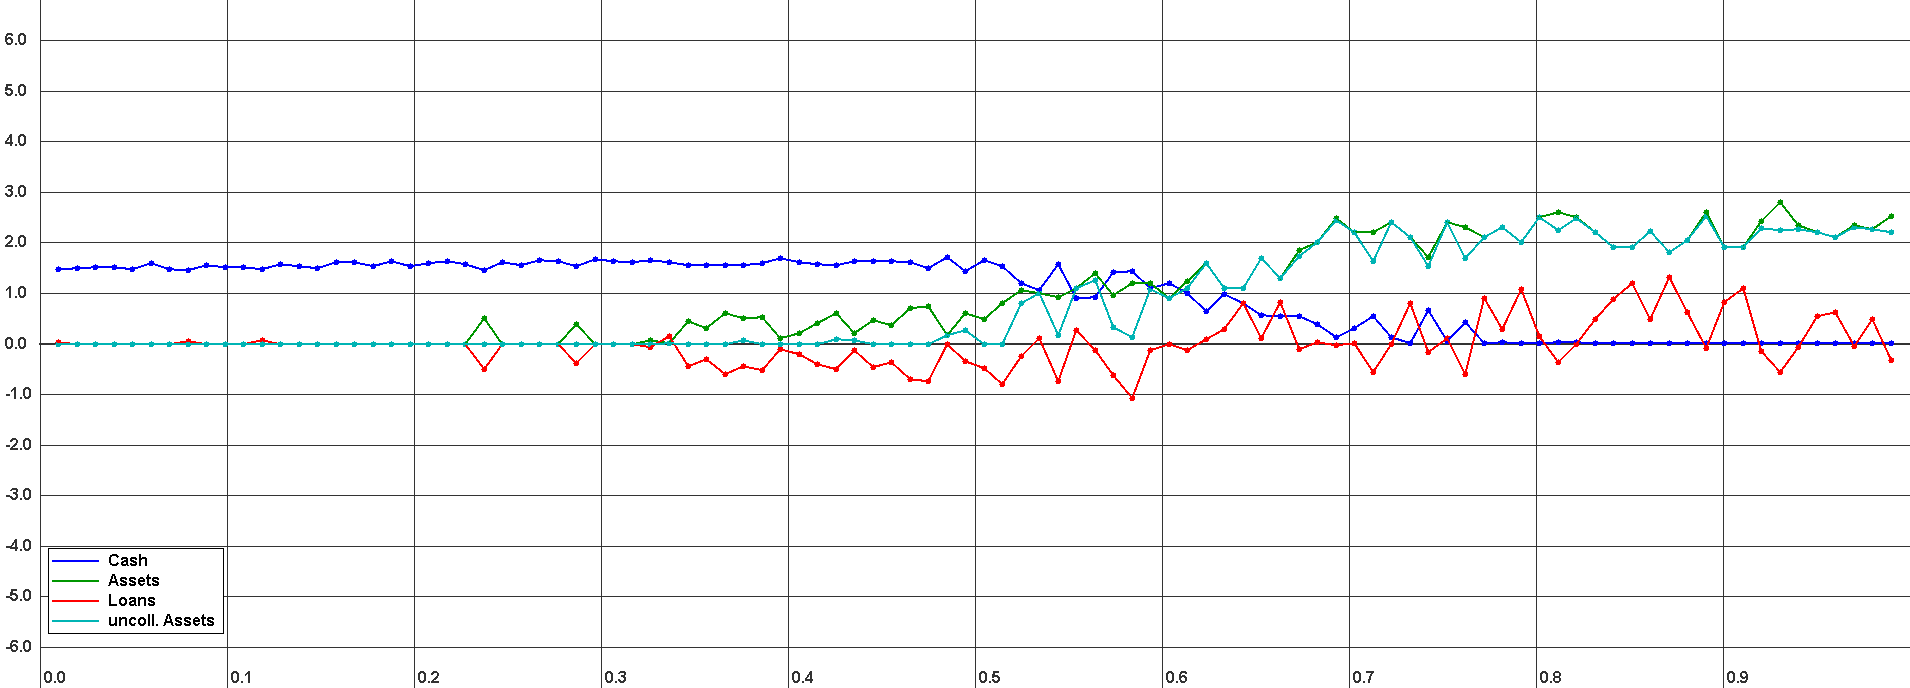
\includegraphics[width=1.0\textwidth, angle=0]{fc/FULLYCONNECTED_100_WITHCOLLATERALMARKET_WEALTH_STAGE_2.png}
  	\caption{Wealth-Distribution of Fully-Connected topology with collateral/cash market during Stage 2}
	\label{fig:markets_FULLYCONNECTED_100_WITHCOLLATERALMARKET_WEALTH_STAGE_2}
\end{figure}

\paragraph{Stage 3}
The pessimists have gone inactive as they hold no more wealth they can trade. The i0-point is emerging and the medianists and pure optimists begin to show up.

\medskip

Because the pessimists are inactive now and hold no more assets the asset/cash and collateral/cash markets go down and declines completely.
The loan/cash market goes down but does not decline.
The medianists and optimists which are emerging have no other possibility than to trade on the asset/loan market to further distribute their collateralized assets among each other which is the reason for the raise of the asset/loan market above all others and its heavy domination.

\begin{figure}[H]
	\centering
  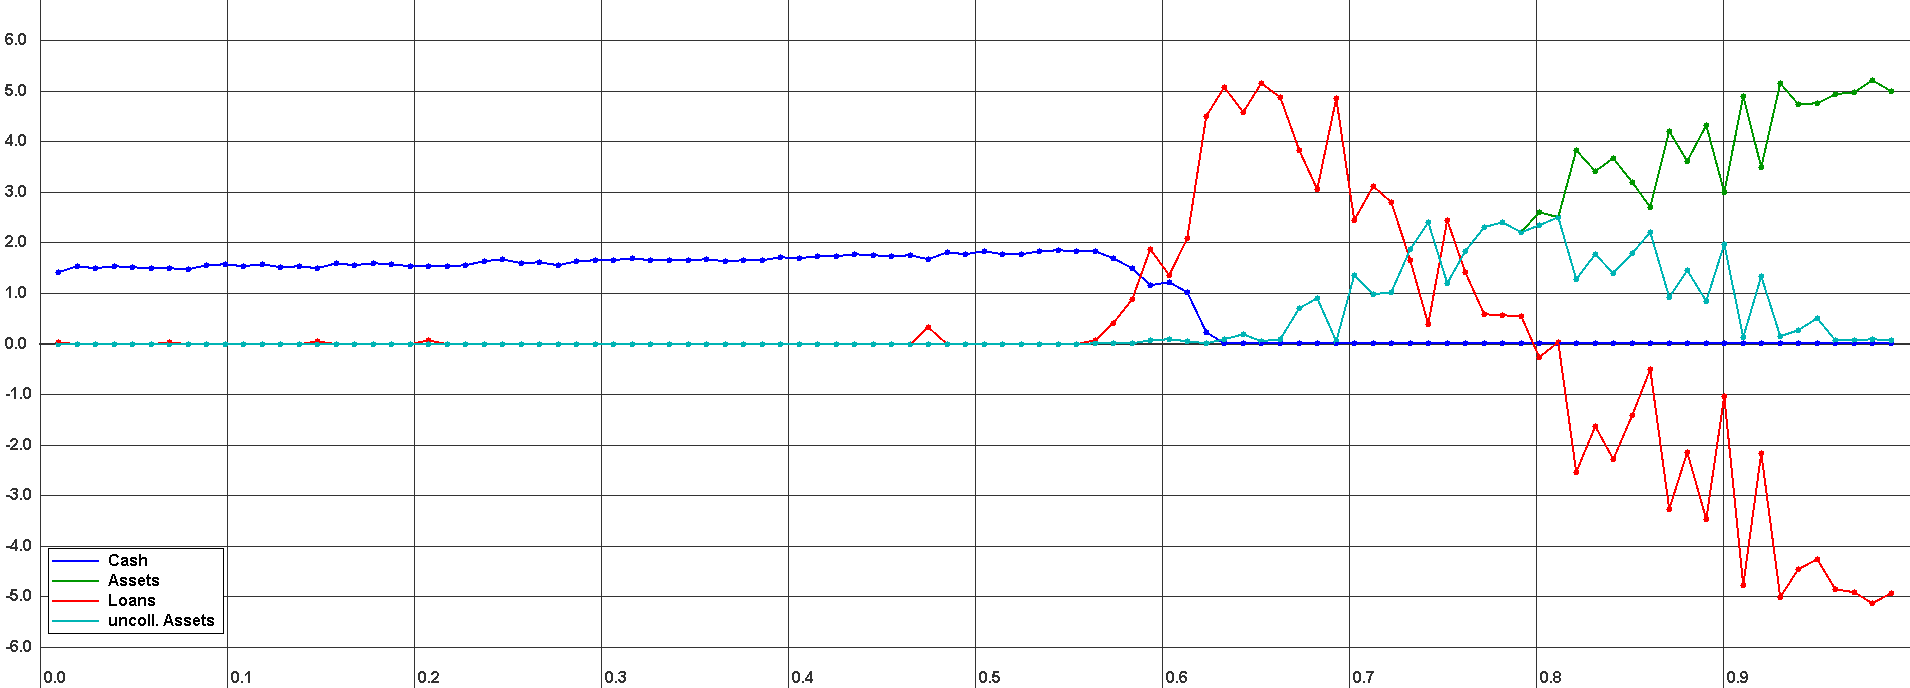
\includegraphics[width=1.0\textwidth, angle=0]{fc/FULLYCONNECTED_100_WITHCOLLATERALMARKET_WEALTH_STAGE_3.png}
  	\caption{Wealth-Distribution of Fully-Connected topology with collateral/cash market during Stage 3}
	\label{fig:markets_FULLYCONNECTED_100_WITHCOLLATERALMARKET_WEALTH_STAGE_3}
\end{figure}

\paragraph{Stage 4}
Finally the i1-point has emerged and both i0 and i1 are finalizing. The only active agents remaining are around these two points where the pure optimists trade with the medianists to finalize i1 and the medianists with the next closest pessimists to finalize i0 where the very last transactions occur around i0.

\medskip

The asset/loan market goes down until i1 has finalized as the collateralized asset allocation has nearly reached its equilibrium.
The loan/cash market goes up as agents around i0 are still refining the point as the equilibrium of the medianists have not yet reached and thus bonds are traded against cash as i0 is the connecting point between pessimists with cash and medianists with bond which enables the loan/cash market to trade again.

\begin{figure}[H]
	\centering
  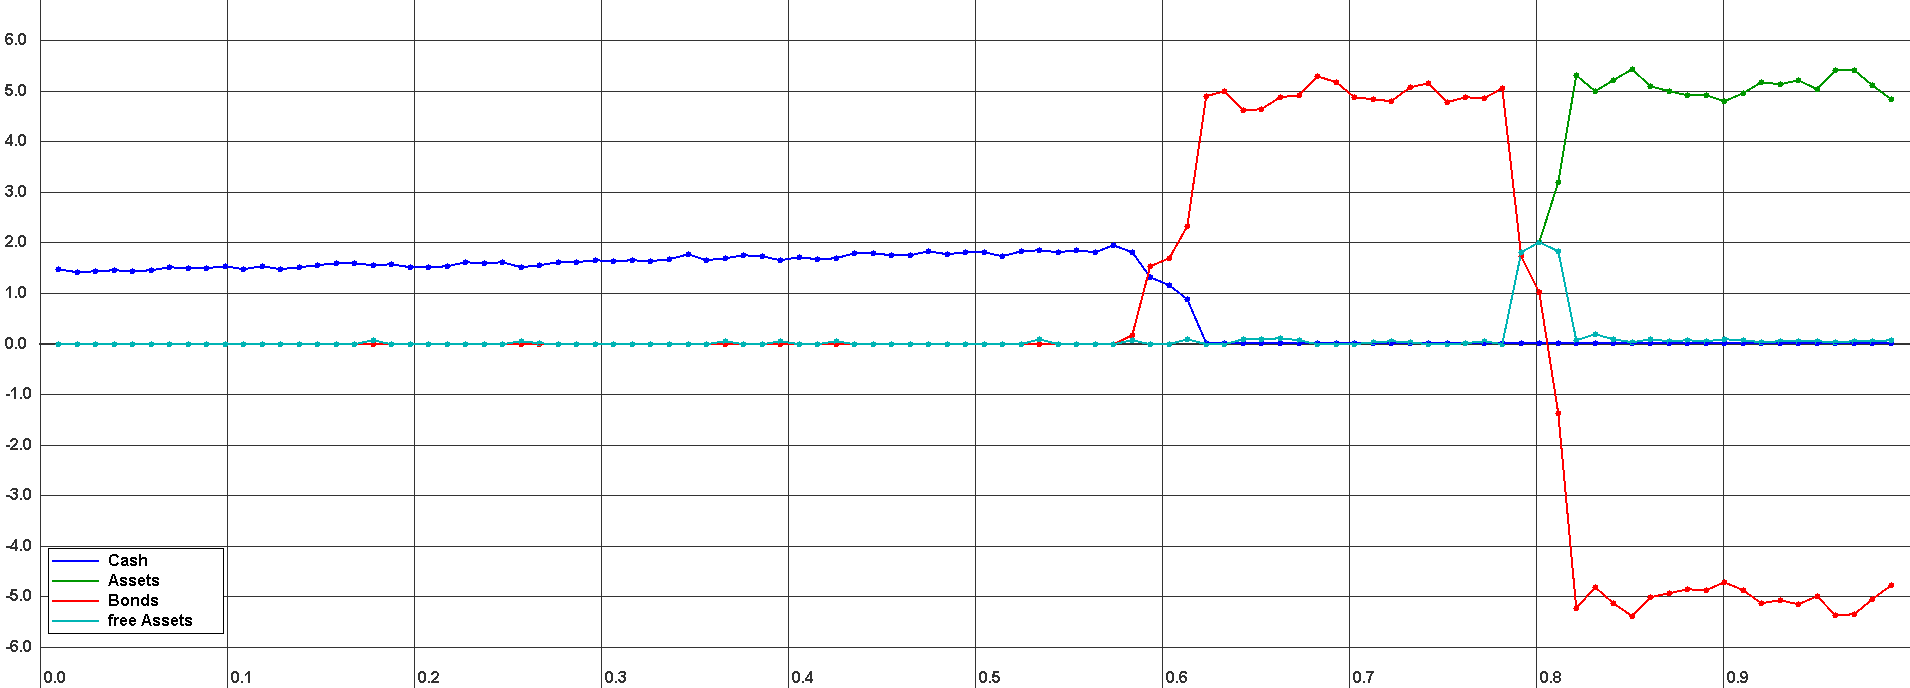
\includegraphics[width=1.0\textwidth, angle=0]{fc/FULLYCONNECTED_100_WITHCOLLATERALMARKET_WEALTH_STAGE_4.png}
  	\caption{Wealth-Distribution of Fully-Connected topology with collateral/cash market during Stage 4}
	\label{fig:markets_FULLYCONNECTED_100_WITHCOLLATERALMARKET_WEALTH_STAGE_4}
\end{figure}

\subsection{Ascending-Connected without new Market}

3 Stages were identified where all of them can be seen in the Market-Dynamics diagram.

\begin{figure}[H]
	\centering
  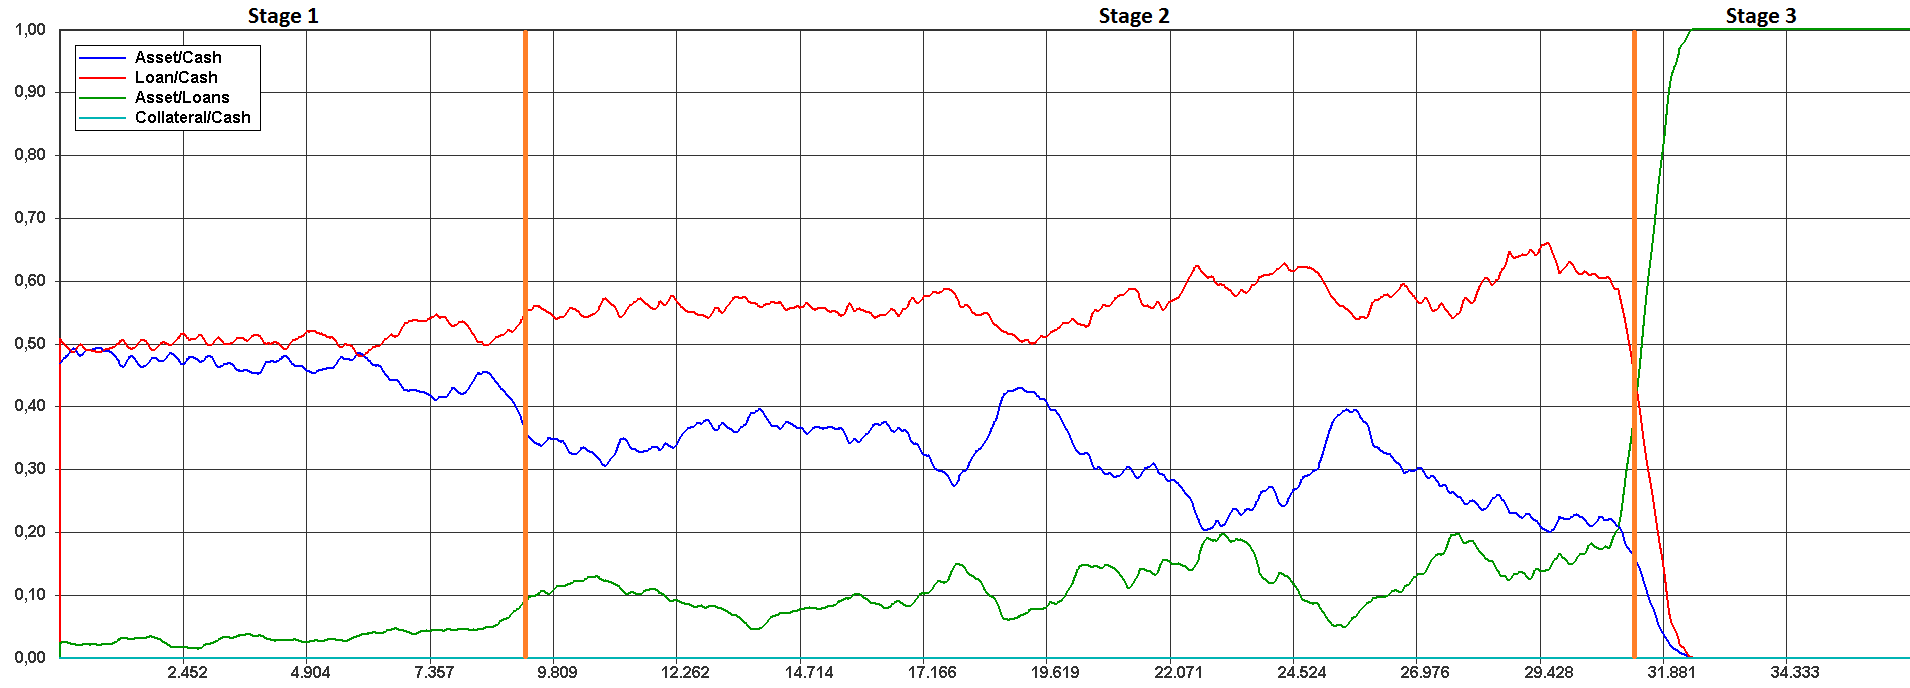
\includegraphics[width=1.0\textwidth, angle=0]{ac/ASCENDINGCONNECTED_100_NOCOLLATERALMARKET_MARKET_STAGES.png}
  	\caption{Market-activity stages of Ascending-Connected topology without collateral/cash market}
	\label{fig:markets_ASCENDINGCONNECTED_100_NOCOLLATERALMARKET_MARKET_STAGES}
\end{figure}

\paragraph{Stage 1}
The allocations are very chaotic overall but pessimists can be identified already as they sell their free assets against cash thus holding primarily cash but lots of collateralized assets are in the pessimists-range as well. Real distinction of optimists is not yet visible and medianists are far from showing up.

\medskip

The asset/cash and loan/cash markets are very dominant in this stage as the pessimists try to get cash for their free assets where the asset/loan market is hardly active but contributes enough to create the miss-allocation of the collateralized assets in the pessimists-range already.

\begin{figure}[H]
	\centering
  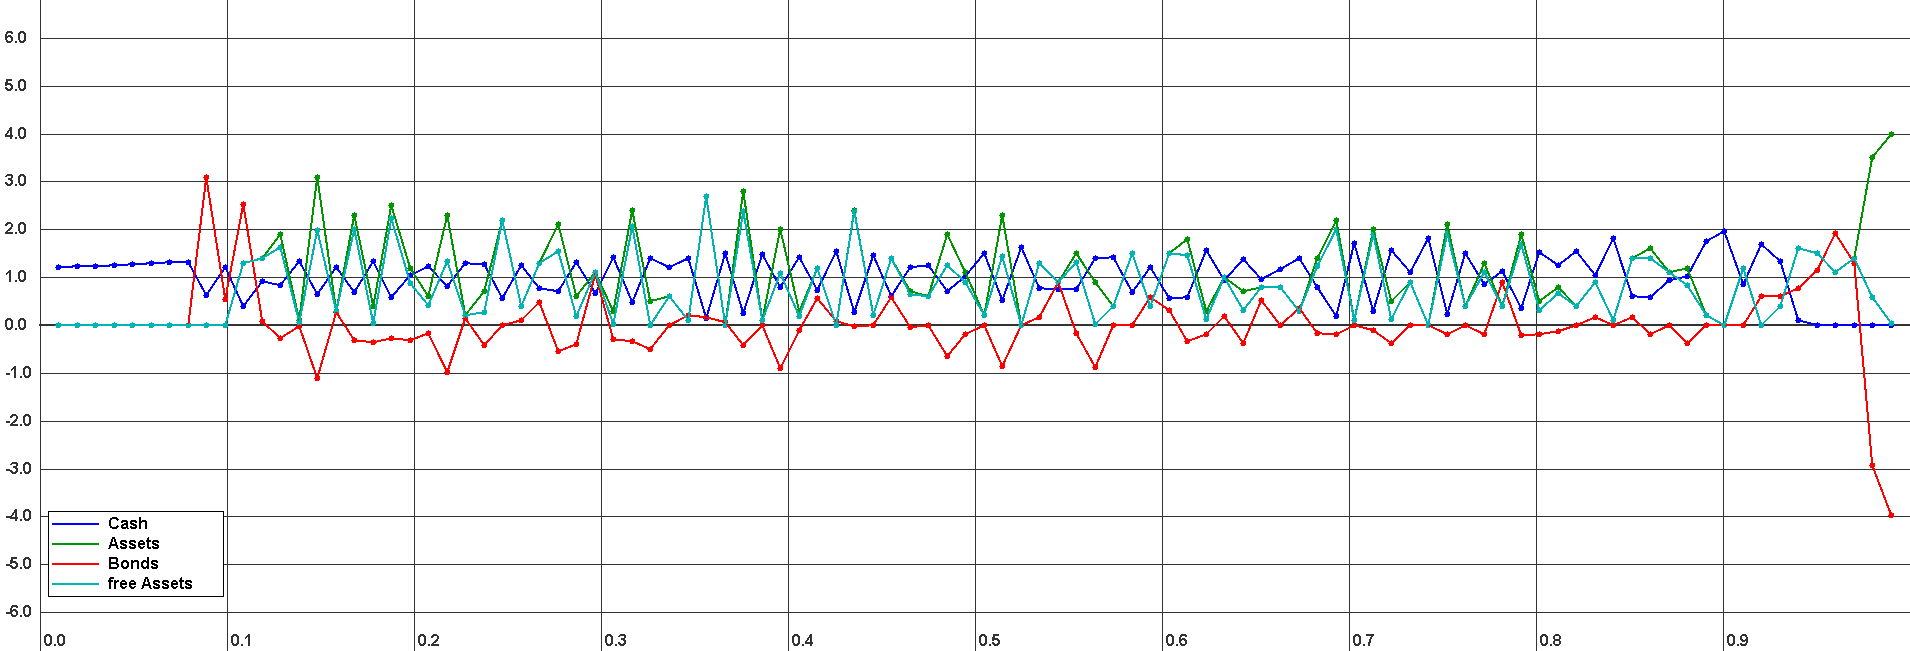
\includegraphics[width=1.0\textwidth, angle=0]{ac/ASCENDINGCONNECTED_100_NOCOLLATERALMARKET_WEALTH_STAGE_1.png}
  	\caption{Wealth-Distribution of Ascending-Connected topology without collateral/cash market during Stage 1}
	\label{fig:markets_ASCENDINGCONNECTED_100_NOCOLLATERALMARKET_WEALTH_STAGE_1}
\end{figure}

\paragraph{Stage 2}
The pessimists which hold collateralized assets try to trade them up to the optimists which looks like waves when visualisizing it in the thesis-software. The optimists are now about to emerge as most of them are maximally short on cash and hold either free or collateralized assets. The medianists are still not visible yet.

\medskip
		
The asset/cash market seems to go down in the long term while the loan/cash and asset/loan markets seems to increase as the fewer assets can be traded against cash and the optimists are already very low on cash thus the asset/loan market is naturally increasing.
		
\begin{figure}[H]
	\centering
  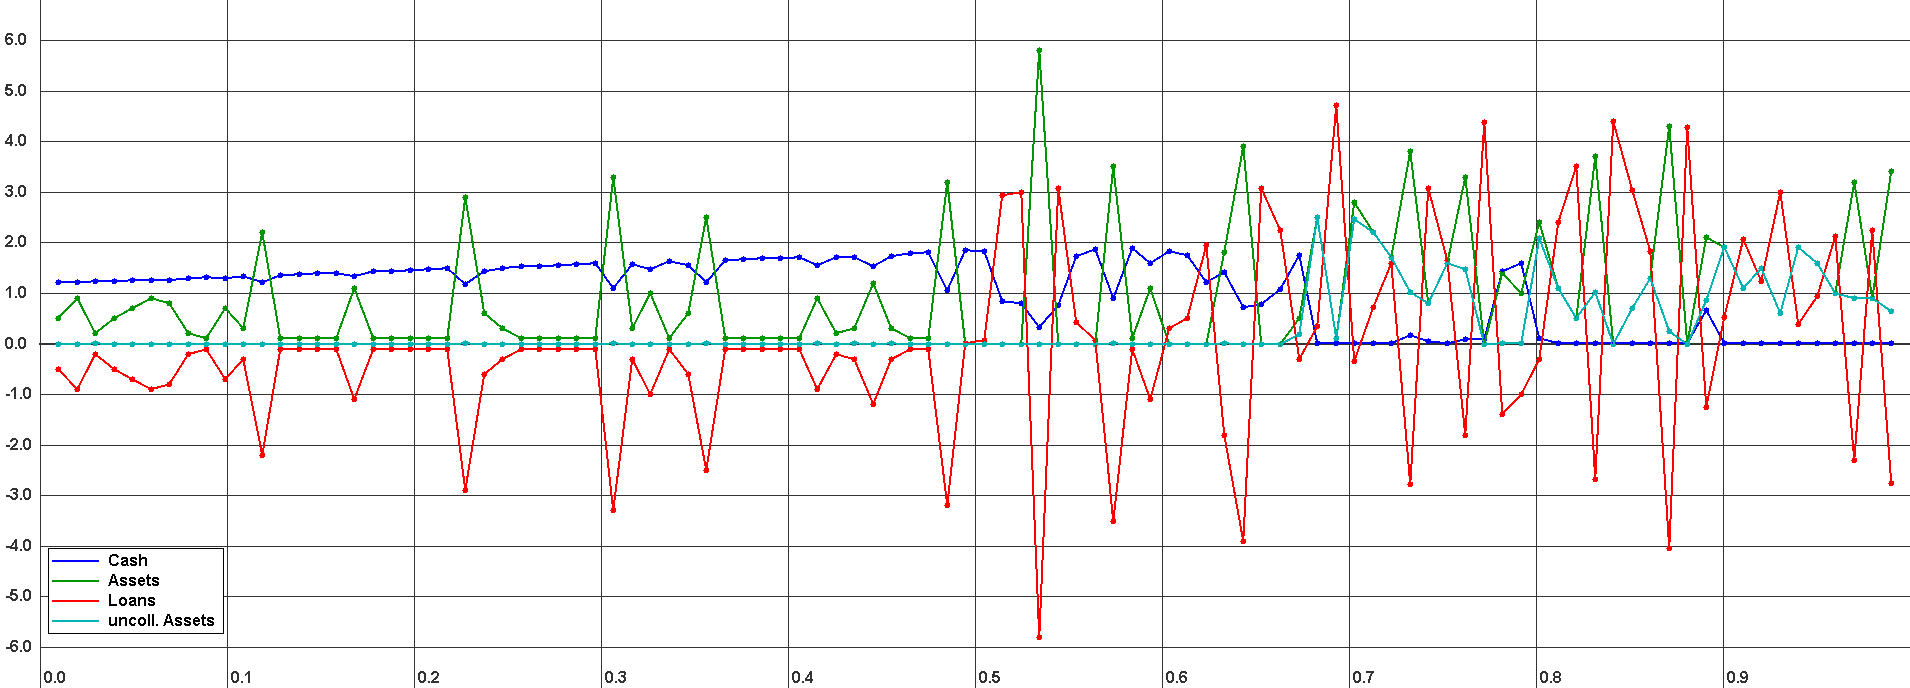
\includegraphics[width=1.0\textwidth, angle=0]{ac/ASCENDINGCONNECTED_100_NOCOLLATERALMARKET_WEALTH_STAGE_2.png}
  	\caption{Wealth-Distribution of Ascending-Connected topology without collateral/cash market during Stage 2}
	\label{fig:markets_ASCENDINGCONNECTED_100_NOCOLLATERALMARKET_WEALTH_STAGE_2}
\end{figure}
		
\paragraph{Stage 3}
The pessimists lie dormant and are completely inactive. The medianists begin to show up holding only bonds and the real optimists begin to cristalize holding only collateralized assets. These two frontiers move towards each other and when they have reached, trading is over and SOME equilibrium is reached

\medskip

The asset/cash market lies dormant as well as because the pessimists are no more able to trade without the new market and the optimists are maximally low on cash. The loan/cash market is inactive too whereas the asset/loan market takes over and dominates 100\% as only collateralized assets are traded on asset/loan market.

\begin{figure}[H]
	\centering
  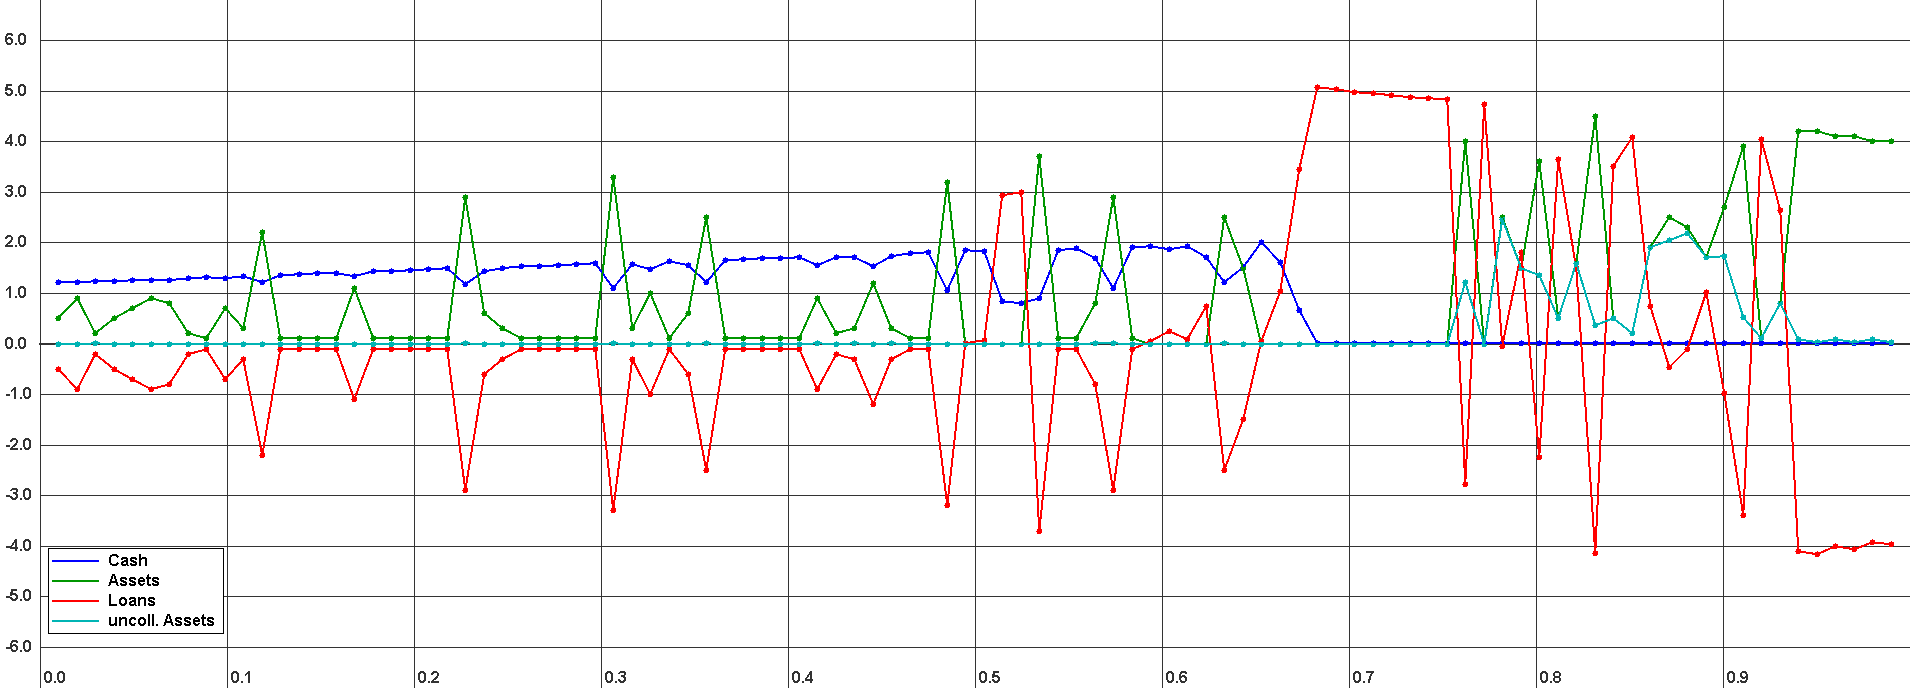
\includegraphics[width=1.0\textwidth, angle=0]{ac/ASCENDINGCONNECTED_100_NOCOLLATERALMARKET_WEALTH_STAGE_3.png}
  	\caption{Wealth-Distribution of Ascending-Connected topology without collateral/cash market during Stage 3}
	\label{fig:markets_ASCENDINGCONNECTED_100_NOCOLLATERALMARKET_WEALTH_STAGE_3}
\end{figure}

\subsection{Ascending-Connected with new Market enabled after 1000 successive failed Transactions}
Using the thesis-software it is possible to start a simulation-run on ascending-connected topology without the collateral/cash market and enabling it after 1000 successive failed transactions which gives interesting hints about how the spikes of collateralized assets in the pessimists-range are resolved and distributed over the already existing pure optimists.

\medskip

Of course there are the same 3 Stages to be found as above whereas the deferred enabling of the collateral/cash market adds 2 new Stages.

\begin{figure}[H]
	\centering
  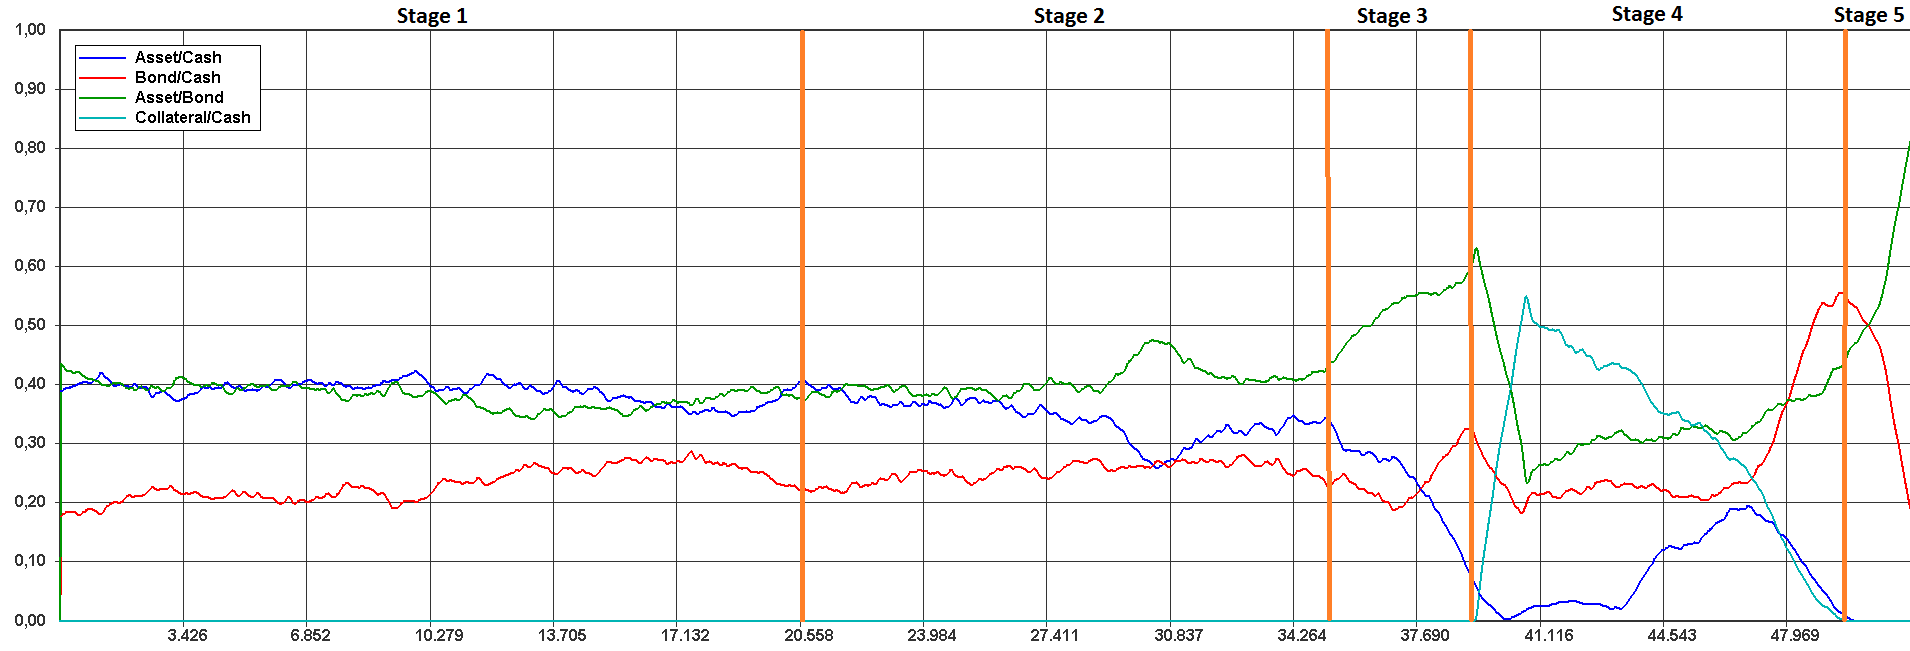
\includegraphics[width=1.0\textwidth, angle=0]{ac/ASCENDINGCONNECTED_100_DEFERREDCOLLATERALMARKET_MARKET_STAGES.png}
  	\caption{Market-activity stages of Ascending-Connected topology with deferred activated collateral/cash market}
	\label{fig:markets_ASCENDINGCONNECTED_100_DEFERREDCOLLATERALMARKET_MARKET_STAGES}
\end{figure}

\paragraph{Stage 4}
The collateralized assets are traded against cash and sum up at the i0-point where the first agent has no more cash. 

\begin{figure}[H]
	\centering
  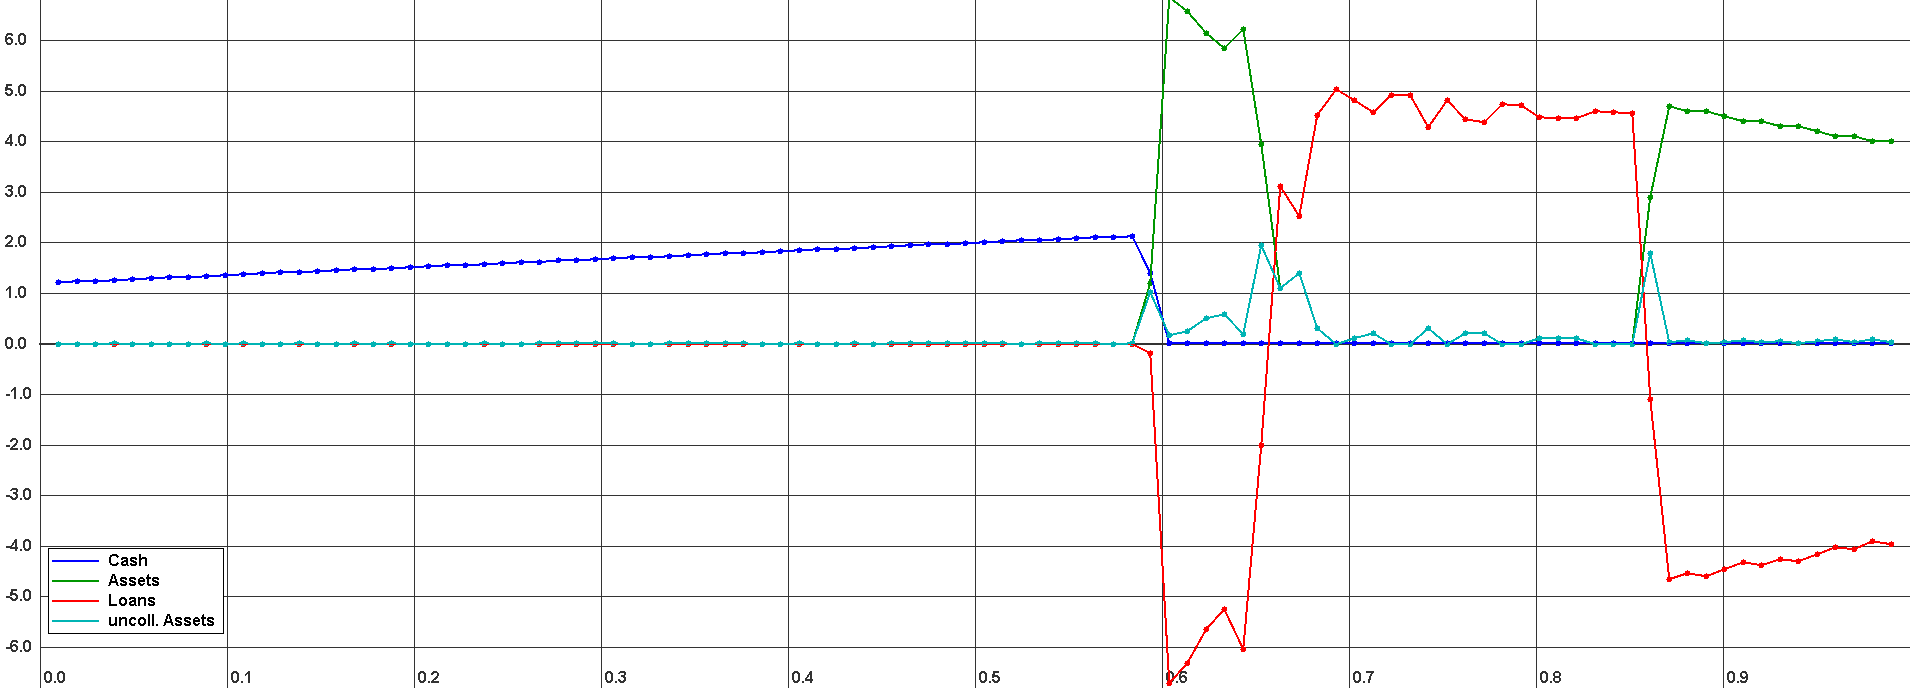
\includegraphics[width=1.0\textwidth, angle=0]{ac/ASCENDINGCONNECTED_100_DEFERREDCOLLATERALMARKET_WEALTH_STAGE_4.png}
  	\caption{Wealth-Distribution of Ascending-Connected topology with deferred activated collateral/cash market during Stage 4}
	\label{fig:markets_ASCENDINGCONNECTED_100_DEFERREDCOLLATERALMARKET_WEALTH_STAGE_4}
\end{figure}

\paragraph{Stage 5}
Now the asset/loan market becomes 100\% dominant again and the collateralized assets are traded through the medianists towards the pure optimists as they have no more cash and can only trade anymore on this remaining active market.

\begin{figure}[H]
	\centering
  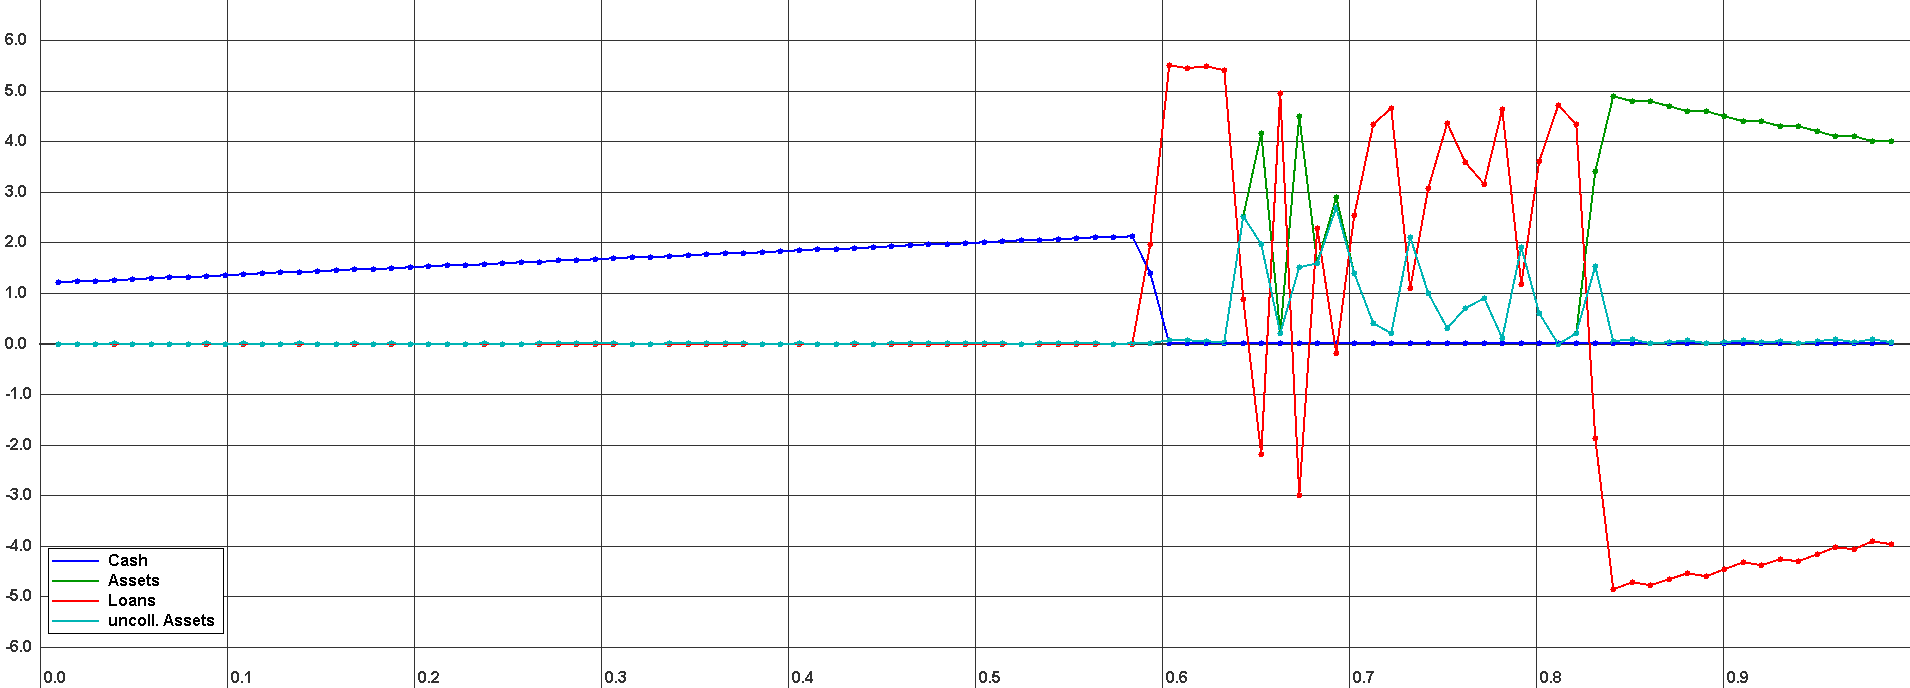
\includegraphics[width=1.0\textwidth, angle=0]{ac/ASCENDINGCONNECTED_100_DEFERREDCOLLATERALMARKET_WEALTH_STAGE_5.png}
  	\caption{Wealth-Distribution of Ascending-Connected topology with deferred activated collateral/cash market during Stage 5}	\label{fig:markets_ASCENDINGCONNECTED_100_DEFERREDCOLLATERALMARKET_WEALTH_STAGE_5}
\end{figure}

\subsection{Ascending-Connected with new Market}

4 Stages were identified where only 3 of them can be seen in the Market-Dynamics diagram.

\begin{figure}[H]
	\centering
  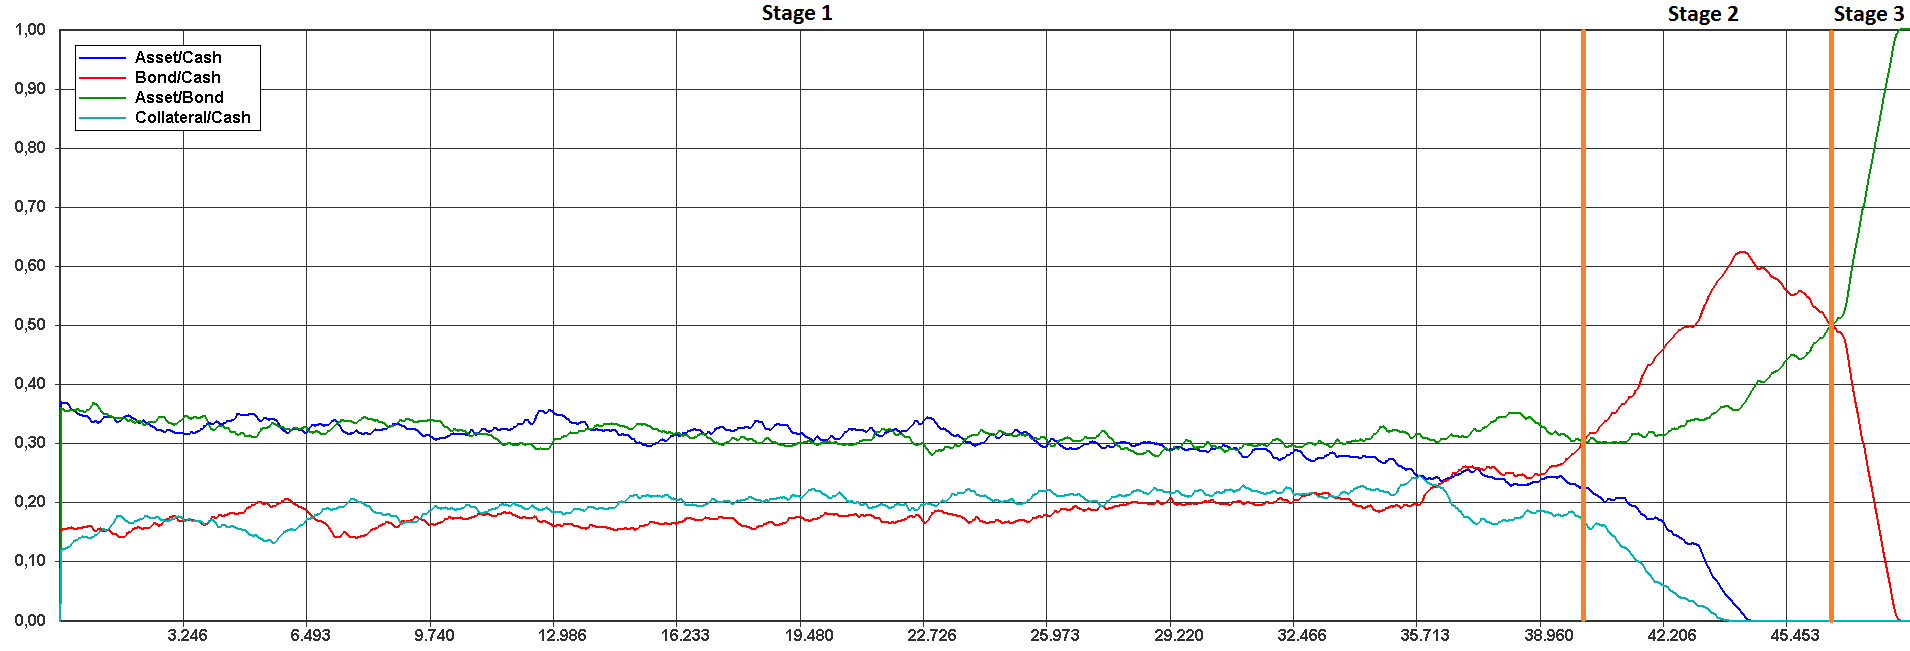
\includegraphics[width=1.0\textwidth, angle=0]{ac/ASCENDINGCONNECTED_100_WITHCOLLATERALMARKET_MARKET_STAGES.png}
  	\caption{Market-activity stages of Ascending-Connected topology with collateral/cash market}
	\label{fig:markets_ASCENDINGCONNECTED_100_WITHCOLLATERALMARKET_MARKET_STAGES}
\end{figure}

\paragraph{Stage 1}
Pessimists and optimists begin to emerge where the pessimists are gathering cash and collateralized assets and the optimists are gathering free assets against cash and a few collateralized assets. There are no medianists visible yet.

\medskip

The asset/cash market and loan/cash market start around 40\% slightly decreasing where the collateral/cash market starts around 10\% with increasing tendency. The asset/loan market is makes 2\% of the total activity. It is clear to see that the collateral/cash market is increasing as the amount of collateralized assets which moves towards the optimists increases.
		
\begin{figure}[H]
	\centering
  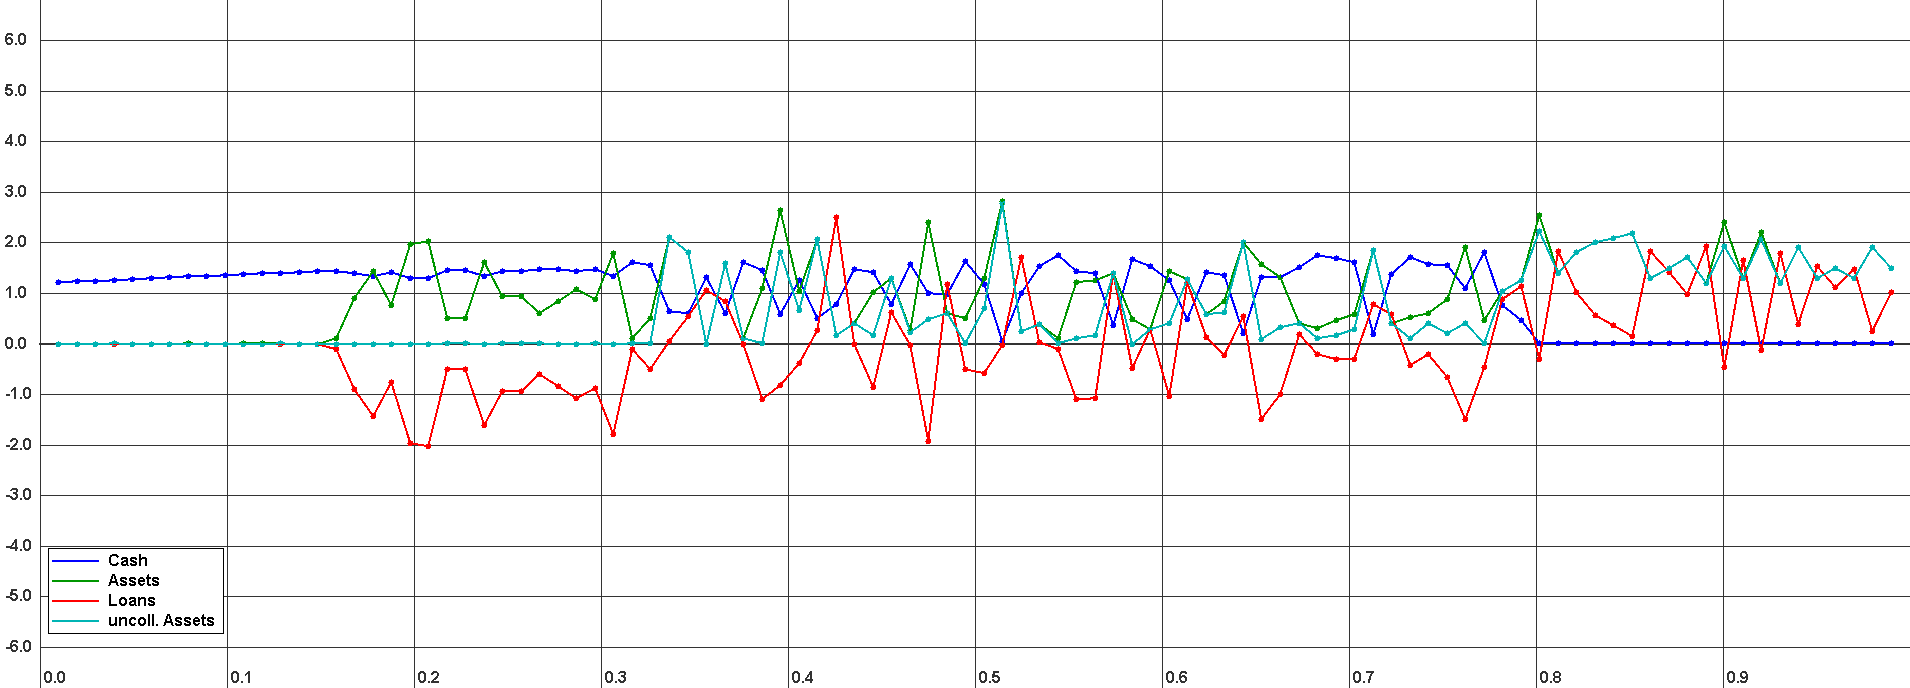
\includegraphics[width=1.0\textwidth, angle=0]{ac/ASCENDINGCONNECTED_100_WITHCOLLATERALMARKET_WEALTH_STAGE_1.png}
  	\caption{Wealth-Distribution of Ascending-Connected topology with collateral/cash market during Stage 1}
	\label{fig:wealth_ASCENDINGCONNECTED_100_WITHCOLLATERALMARKET_WEALTH_STAGE_1}
\end{figure}

\paragraph{Stage 2}
In the pessimist-range large amount of collateralized assets have gathered which are traded now towards the optimists as the pessimists try to get maximally short on any assets and maximally plus on cash. Those collateralized assets are traded towards the i0-point - that is the first agent who holds no more cash - which can be seen by a spike in the wealth-distribution of figure \ref{fig:wealth_ASCENDINGCONNECTED_100_WITHCOLLATERALMARKET_WEALTH_STAGE_2} around 0.65.
There are no medianists visible yet.

\medskip

The collateral/cash market raises above the asset/cash and loan/cash markets and either fluctuates or stays quite constant. In figure \ref{fig:markets_ASCENDINGCONNECTED_100_WITHCOLLATERALMARKET_MARKET_STAGES} the fluctuating variant is shown. If the market fluctuates the asset/cash and loan/cash fluctuate inverse in that if collateral/cash market raises they go down and vice versa. If the collateral/cash market stays quite constant in this stage it raises above 90\% and asset/cash and loan/cash markets decline to 0\%. Why the collateral/cash market either fluctuates or stays constant is not clear but is most probably dependent on the allocation of collateralized assets in the pessimists-range. The asset/loan market becomes a bit more active as more collateralized assets are traded.
		
\begin{figure}[H]
	\centering
  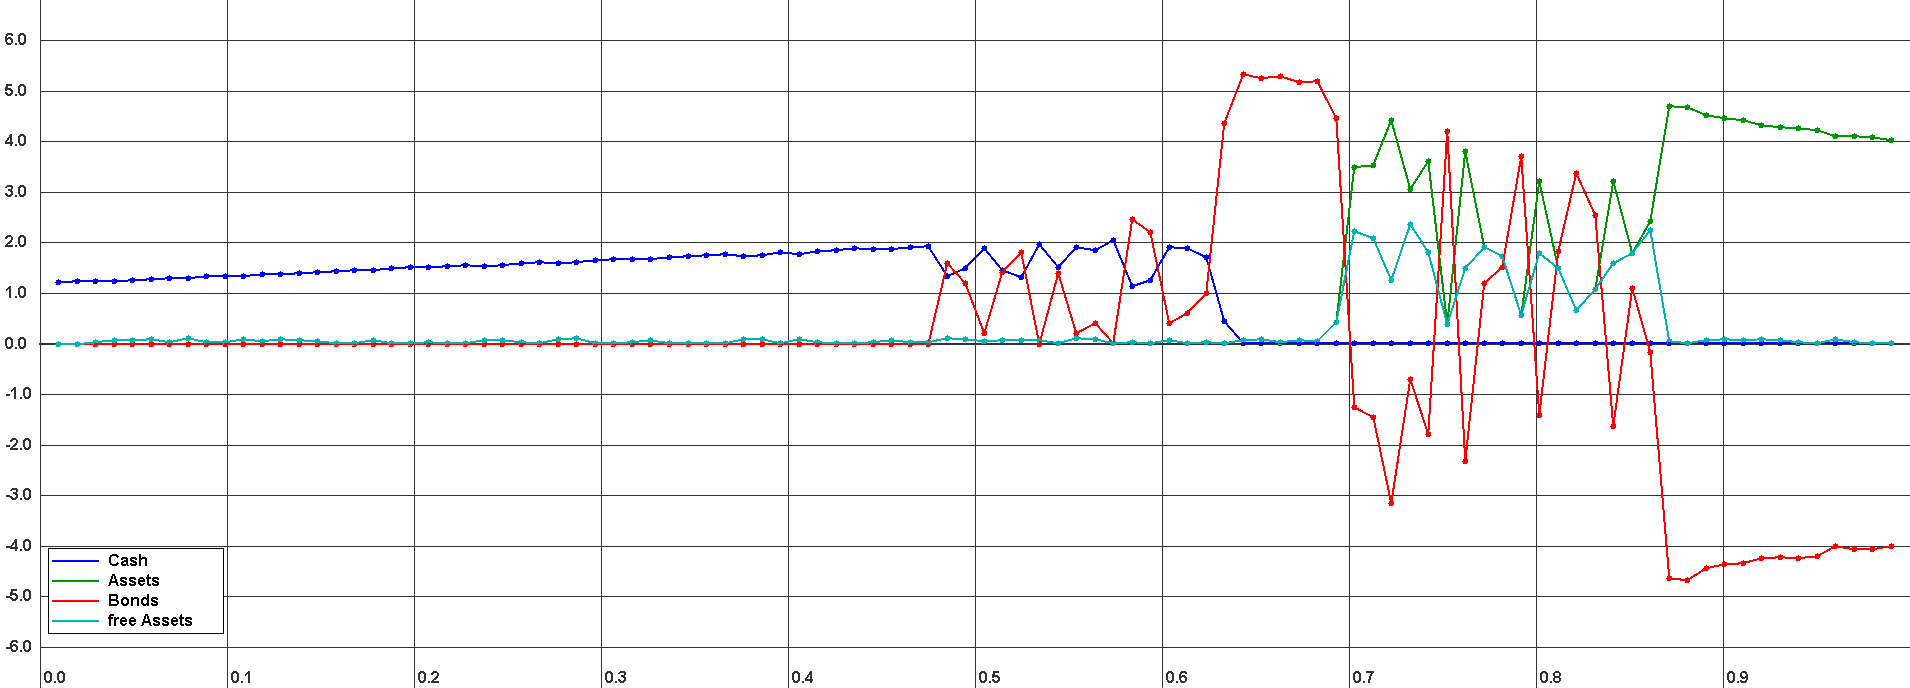
\includegraphics[width=1.0\textwidth, angle=0]{ac/ASCENDINGCONNECTED_100_WITHCOLLATERALMARKET_WEALTH_STAGE_2.png}
  	\caption{Wealth-Distribution of Ascending-Connected topology with collateral/cash market during Stage 2}
	\label{fig:wealth_ASCENDINGCONNECTED_100_WITHCOLLATERALMARKET_WEALTH_STAGE_2}
\end{figure}

\paragraph{Stage 3}
Pessimists are now final and won't change any more. Optimists-range is now clearly visible and holds a large amount of collateralized assets from the pessimists which needs now to be traded and distributed to the remaining optimists. Medianists are still not visible yet.

\medskip

Because the pessimists are no more able to trade and the optimists hold no more cash the activity of the collateral/cash market drops rapidly and asset/loan market raises to 100\% activity as only collateralized-assets are tradeable any more.
		
\begin{figure}[H]
	\centering
  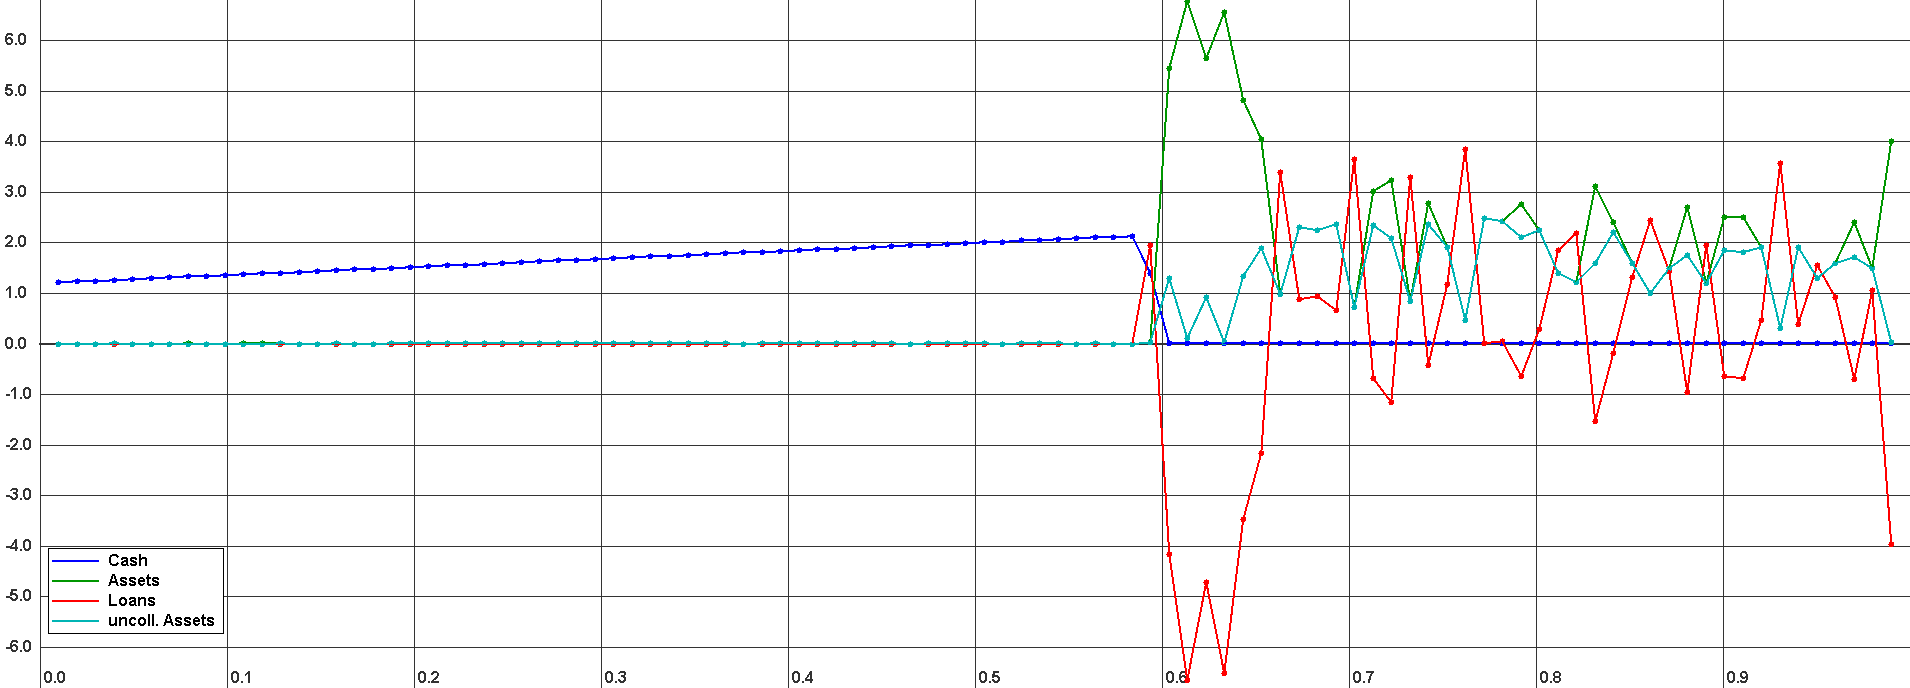
\includegraphics[width=1.0\textwidth, angle=0]{ac/ASCENDINGCONNECTED_100_WITHCOLLATERALMARKET_WEALTH_STAGE_3.png}
  	\caption{Wealth-Distribution of Ascending-Connected topology with collateral/cash market during Stage 3}
	\label{fig:wealth_ASCENDINGCONNECTED_100_WITHCOLLATERALMARKET_WEALTH_STAGE_3}
\end{figure}

\paragraph{Stage 4}
Medianists begin to show up and to distinguish themselves from the pure optimists. This is no more visible on the market-dynamics as only asset/bonds are traded anymore.
		
\begin{figure}[H]
	\centering
  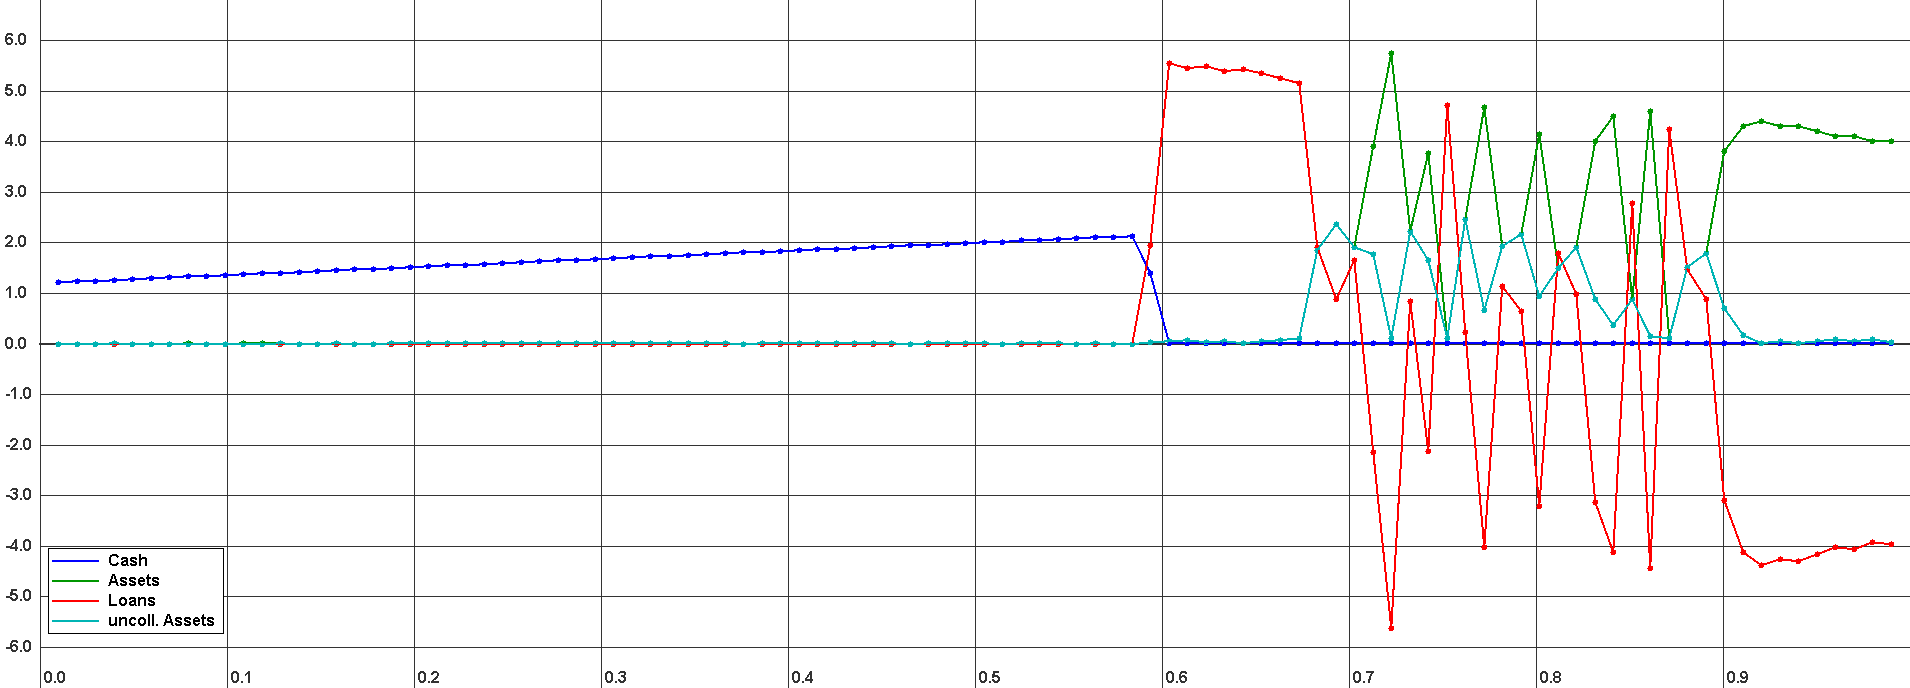
\includegraphics[width=1.0\textwidth, angle=0]{ac/ASCENDINGCONNECTED_100_WITHCOLLATERALMARKET_WEALTH_STAGE_4.png}
  	\caption{Wealth-Distribution of Ascending-Connected topology with collateral/cash market during Stage 4}
	\label{fig:wealth_ASCENDINGCONNECTED_100_WITHCOLLATERALMARKET_WEALTH_STAGE_4}
\end{figure}


\paragraph{How does trading progress with this new market? Is it the same as without the new market?}
TODO. vermutung: gleich, aber es wird halt auch noch der neue markt verwendet

\paragraph{How does the new market resolve the miss-allocation?}
TODO nocheinmal die dynamiken untersuchen: wie passiert schlussendlich das unkollateralisieren von assets? die kollateralisierten assets werden ja nicht unkollateralisiert sondern wandern einfach zu den optimisten. unkollateralisiert werden sie ja nicht. die medianisten haben keinen cash mehr und kaufen assets gegen bonds und unkollateralisieren sie. genau erklären.

\paragraph{Can the trading stages 1-4 be identified too as given in \cite{Breuer_2015}?}



\section{Conclusions on new Market}
The equilibrium of the ascending-connected topology with the new market is different than the fully-connected one which reaches the theoretical equilibrium. Thus the hypothesis is still wrong because it predicted the ascending-connected topology to reach the theoretical equilibrium. This thesis can only speculate on the real reason for this but the reason is most probably rooted in the fundamental different trading dynamics of ascending-connected topology compared to fully-connected as can be seen in the market-dynamics. This thesis leaves this question open for further research.

\end{document}
